%%%%%%%%%%%%%%%%%%%%%%%%%%%%%%%%%%%%%%%%%%%%%%%%%%%%%%%%%%%%%%%%%%%%%%
% Lớp 11 | Đường thẳng, mặt phẳng. Quan hệ song song trong | Hai đường thẳng song song
% Dạng 1H4?2-3: Tìm giao tuyến bằng cách kẻ song song
% Số câu: 37  (sinh tự động bởi tach_cau.py; từ nay thầy sửa trực tiếp file này)
%%%%%%%%%%%%%%%%%%%%%%%%%%%%%%%%%%%%%%%%%%%%%%%%%%%%%%%%%%%%%%%%%%%%%%

%%%%%%%%%%%%%%%% TRẮC NGHIỆM 4 PHƯƠNG ÁN %%%%%%%%%%%%%%%%

% nguồn: Ok_TracNghiemLop11_Lan1
\begin{ex}%[1H4N2-3]%[ma:916faa7b]
	Cho hình chóp $S.ABCD$ có đáy $ABCD$ là hình bình hành. Giao tuyến của hai mặt phẳng $(SAB)$ và $(SCD)$  là đường thẳng song song với đường thẳng nào sau đây?
	 \choice
		{$BD$ } 
		 {$SC$}
		 {$AC$}
		{\True  $AB$}
	\loigiai{ 
	\immini{Ta có  $\heva{&S\in (SAB)\cap (SCD) \\&AB\parallel CD\\&AB\subset (SAB)\\&CD\subset(SCD)}$\\
		$\Rightarrow Sx=(SAB)\cap (SCD)\quad  $(với $Sx \parallel AB\parallel CD$).}
		{	\begin{tikzpicture}[line join=round,line cap=round,scale=.7]
		\coordinate (S)  at (0,4);
		\coordinate (A)  at (0,0);
		\coordinate (D)  at (-2,-2);
		\coordinate (C) at  (3,-2);
		\coordinate  (B) at (5,0);
		 \coordinate (E) at (-2,4);
		\coordinate (F)  at (5,4);
		\draw  (S)--(B)
			(S)--(C) 
			 (S)--(D)
			(B)--(C) 
			(C)--(D) 
			(E)--(F) node[below]{$x$}; 
		 \draw[dashed](A)--(D)
			(S)--(A) 
			 (A)--(B);
		\foreach \i/\g in {S/90,A/180,B/-80,C/-80,D/180}{\draw[fill](\i) circle (1pt) 
			($(\i)+(\g:3mm)$)  node[scale=1]{$\i$};}
	\end{tikzpicture}
		 }
	 }
\end{ex}

% nguồn: Ok_Toan11_TracNghiem_Lan2
\begin{ex}%[1H4H2-3]%[ma:2d6a4962]
	Cho tứ  diện $ABCD$. Gọi $M$, $N$, $P$, $Q$ lần lượt là trung điểm của các cạnh $AB$, $AD$, $CD$, $BC$. Tìm điều kiện để $MNPQ$ là hình thoi.
	 \choice
		{$AB=BC$} 
		 {$BC=AD$}
		 {\True $AC=BD$}
		 {$AB=CD$}
	\loigiai{ 
		\begin{center}
			\begin{tikzpicture}[declare function={goc=-45; a=5; b=0.45*a; h=5;}]
					 \path
						(0,0)  coordinate (B)
						 (a,0) coordinate (D)
						 (goc:b) coordinate (C)--+(0,h) coordinate (A)
						 ($(A)!.5!(B)$) coordinate (M)
						($(A)!.5!(D)$) coordinate (N) 
						($(C)!.5!(D)$) coordinate (P) 
						($(C)!.5!(B)$) coordinate  (Q);
					 \draw[dashed] (B)--(D)
						 (M)--(N)
						 (P)--(Q);
					\draw (A)--(C) 
						(A)--(B)--(C)--(D)--cycle (M)--(Q) 
						 (N)--(P);
					\foreach \x/\goc in {D/0,A/90,C/-60,B/180,M/180,N/20,P/0,Q/180} 
					\draw[fill=white] (\x)  node[shift={(\goc:7pt)},font=\scriptsize]{$\x$} circle (1pt);
				\end{tikzpicture}
		\end{center}
		Xét tam giác $ABD$ có $MN$ là đường trung bình nên $MN\parallel  BD$, $MN=\dfrac{1}{2}BD$.\\
		Tương tự tam giác $BCD$, có $PQ$ là đường trung bình  nên $PQ\parallel BD$, $ PQ=\dfrac{1}{2}BD$.\\
		Tứ giác $MNPQ$ có $MN\parallel PQ$, $MN=PQ$ suy ra  tứ giác $MNPQ$ là hình bình hành.\\
		Để $MNPQ$ là hình  thoi thì $MN=MQ$ hay $BD=AC$.
	} 
\end{ex}

% nguồn: Ok_Toan11_TracNghiem_Lan2
\begin{ex}%[1H4H2-3]%[ma:cae5d75f]
	Cho hình chóp $S.ABC$. Gọi $M$ và $N$ lần lượt là trung điểm của $ AB$ và $ AC$. Giao tuyến của hai mặt phẳng $(SMN)$ và $(SBC)$ là một đường thẳng song song với đường thẳng nào sau đây? 
	 \choice
		 {$AC$}
		{\True $BC$} 
		 {$AB$}
		 {$SA$}
	 \loigiai{
		\begin{center}
			\begin{tikzpicture}[declare function={goc=-55; a=5; b=0.45*a; h=5;}]
					\path 
						(0,0) coordinate (A) 
						(a,0)  coordinate (C)
						(goc:b)  coordinate (B)
						($(A)!.5!(B)$)  coordinate (M)
						($(A)!.5!(C)$)  coordinate (N)
						 +(0,h) coordinate (S);
					\draw[dashed] (M)--(N)--(S) 
						 (A)--(C);
					 \draw (S)--(B)
						 (S)--(A)--(B)--(C)--cycle (M)--(S);
					\foreach  \x/\goc in {S/90,A/180,C/0,B/-90,M/180,N/40}
					 \draw[fill=black] (\x) node[shift={(\goc:7pt)},font=\scriptsize]{$\x$} circle (1pt);
				\end{tikzpicture}
		\end{center}
		Xét $\triangle ABC$ có $ M$ và $ N$ lần lượt là trung điểm của $ AB$ và $ AC$ nên $ MN$ là đường trung bình suy ra $ MN\parallel  BC$.\\
		Ta có $\left\{\begin{array}{l}
		 S\in\left(SMN\right)\cap\left(SBC\right)\\
		MN\subset\left(SMN\right);\,BC\subset\left(SBC\right)\\ 
		 MN\parallel BC
	\end{array}\right.\Rightarrow $$\left(SMN\right)\cap\left(SBC\right)=Sx\parallel MN\parallel BC$.
	} 
\end{ex}

% nguồn: Ok_TracNghiemLop11_Lan1
\begin{ex}%[1H4H2-3]%[ma:642e5998]
	Cho hình chóp $S.ABCD$ có đáy $ABCD$ là hình bình hành. Gọi $M$, $N$ lần lượt là  trung điểm của $SB$, $SD$. Khi đó giao tuyến của hai mặt phẳng $\left(CMN\right)$ và $\left(ABCD\right)$ là
	 \choice
		{đường thẳng $CI$, với  $I=MN\cap BD$}
		{đường  thẳng $MN$}
		 {đường thẳng $BD$}
		{\True đường thẳng $d$ đi qua $C$ và  $d\parallel BD$}
	 \loigiai{
	\immini{ 
		Ta có $\heva{&C\in(CMN)\cap(ABCD)\\&MN\parallel BD \text{ (do $MN$ là đường trung bình của $\triangle SBD$)}\\&MN\subset(CMN), BD\subset(ABCD).}$ 
		Suy ra $(CMN)\cap (ABCD)=d$ đi qua $C$ và $d\parallel BD$. 
		}{\begin{tikzpicture}[line join=round,line cap=round,>=stealth,scale=0.5,font=\footnotesize]
		\tikzset{every  node/.style={outer sep=-0.5mm}}
		\foreach \x/\y/\n  in {0/0/A,-2.5/-2/B,6/0/D} \coordinate (\n) at (\x,\y);
		\coordinate (C) at  ($(B)+(D)-(A)$);
		\coordinate  (O) at ($(B)!0.5!(D)$);
		\coordinate  (S) at ($(O)+(-1,5.5)$);
		 \coordinate (M) at ($(B)!0.5!(S)$);
		\coordinate (N) at  ($(D)!0.5!(S)$);
		\draw[thin,dashed]  (B)--(A)--(D)
			(S)--(A) 
			(M)--(N); 
		\draw (S)--(B)--(C)--(D)--(S)--(C) 
			(M)--(C)--(N); 
		\foreach \n/\l in {A/above left,B/below left,C/below  right,D/above right,S/above,M/above left,N/above right} \fill (\n) node[\l]{$\n$} circle (1.75pt);
	\end{tikzpicture}
		 }
	 }
\end{ex}


%%%%%%%%%%%%%%%% ĐÚNG/SAI %%%%%%%%%%%%%%%%

% nguồn: Ok_dungsai_lop11_Lan1
\begin{ex}%[1H4H2-3]%[ma:ec15246d]
 Cho hình chóp $S.ABCD$ có đáy $ABCD$ là hình thang, $AD\parallel BC$ và $AD=2BC$. Gọi $O$ là giao điểm của $AC$ và $BD$, $E$ là điểm trên cạnh $AD$ sao cho  $ED=2EA$ và $N$ là điểm trên cạnh $SD$ sao cho $ND=2NS$. Khi đó
 \choiceTF 
  {\True  $BC\parallel (SAD)$}
  {Giao tuyến của hai mặt phẳng $(SBC)$ và $(SAD)$ đường thẳng qua $S$ và song song với $AB$} 
  {\True Hai mặt phẳng $(OEN)$ và $(SAB)$ song song với nhau} 
  {Gọi $F$ là giao điểm của đường thẳng $SC$ và  mặt phẳng $(OEN)$. Tỉ số $\dfrac{SF}{SC}=\dfrac{1}{2}$}
 \loigiai{ 
  \begin{center}
   \begin{tikzpicture}[scale=1,font=\footnotesize,line join=round,line cap=round,>=stealth]
      \def\h{3}
     \path (0,0) coordinate (A) 
      (-1.2,-1.4) coordinate (B)  ++(0:4) coordinate (C)
       ($(A)+2*(C)-2*(B)$) coordinate (D)
      ($(A)!1/3!(D)$) coordinate (E) 
      (intersection  cs: first line = {(A)--(C)},second line = {(B)--(D)}) coordinate (O)
      (0.5,\h) coordinate (S) 
       ($(S)!1/3!(D)$) coordinate (N)
      ($(C)!1/3!(B)$)  coordinate (M)
      ($(C)!1/3!(S)$) coordinate  (F);
     \draw (S)--(B)--(C)--(D)--(S)--(C) 
       (N)--(F)--(M);
     \draw[dashed]  (O)--(S)--(A)--(B)--(D)--(A)--(C)
      (O)--(E)--(N)--cycle (O)--(M); 
      \draw ($(S)+(0:6)$) coordinate (S1) node[above left]{$x$}--($(S)+(180:6/3)$) coordinate (S2);
     \foreach \i/\j in  {S/90,A/170,B/-90,C/-90,D/0,O/-90,E/40,N/70,F/80,M/-90} \fill (\i) node[shift={(\j:0.3)}]{$\i$} circle (1pt);
    \end{tikzpicture}
  \end{center}
  \begin{itemchoice}
   \itemch \textbf{Đúng}.\\ Ta có $BC\not\subset (SAD)$, $BC\parallel AD$, $AD\subset (SAD)$  nên $BC\parallel (SAD)$.
   \itemch \textbf{Sai}.\\ Ta có $\heva{&S \in(SBC) \cap(SAD) \\& BC \subset(SBC); AD \subset(SAD)\\& BC \parallel AD}\Rightarrow Sx=(SAB) \cap(SCD)$,  $Sx \parallel BC \parallel AD$.
    \itemch \textbf{Đúng}.\\ Trong mặt phẳng $(ABCD)$, gọi $\{M\}=EO\cap BC$. Ta có $\triangle AOD\backsim\triangle COB$ (g.g), do đó
   \[\dfrac{AO}{CO}=\dfrac{AD}{BC}=2  \Rightarrow \dfrac{CO}{CA}=\dfrac{1}{3}.\]
    Lại có $\triangle AEO\backsim\triangle CMO$, $AE=\dfrac{1}{3}AD=\dfrac{2}{3}BC$ nên $\dfrac{CM}{AE}=\dfrac{CO}{AO}=\dfrac{1}{2} \Rightarrow \dfrac{CM}{BC}=\dfrac{1}{3}$.\\
   Xét $\triangle ABC$,  ta có $\dfrac{CO}{CA} =\dfrac{CM}{CB} = \dfrac{1}{3}$ nên $OM\parallel AB$ hay $OE\parallel AB \Rightarrow OE\parallel (SAB)$. \hfill $(1)$\\
   Xét $\triangle SAD$, từ  giả thiết suy ra $\dfrac{DE}{DA} =\dfrac{DN}{DS} = \dfrac{2}{3}$ nên $EN\parallel AS \Rightarrow EN\parallel (SAB)$. \hfill $(2)$\\
   Từ $(1)$ và $(2)$ suy ra $(OEN)\parallel (SAB)$. 
    \itemch \textbf{Sai}.
   Ta có $\{F\}=SC\cap (OEN)$, $\{M\}=BC\cap (OEN)$ nên $MF$ là giao tuyến của hai mặt phẳng $(OEN)$ và $(SBC)$.\\ 
   Lại có $SB$ là giao tuyến của $(SAB)$ và $(SBC)$, $(OEN)\parallel  (SAB)$ nên $MF\parallel BS$.\\
   Trong tam giác $SBC$, có $M\in BC$, $F\in SC$ và $MF\parallel BS$ nên theo định lý Ta-lét  ta có
   \[\dfrac{SF}{SC}=\dfrac{BM}{BC}  = \dfrac{BC-MC}{BC}=1-\dfrac{1}{3}=\dfrac{2}{3}.\]
   Vậy $F$  là điểm nằm trên đoạn $SC$ sao cho $\dfrac{SF}{SC}=\dfrac{2}{3}$.
  \end{itemchoice}
 } 
\end{ex}

% nguồn: Ok_dungsai_lop11_Lan1
\begin{ex}%[1H4H2-3]%[ma:f28f9d50]
 Cho hình chóp $S.ABCD$ có đáy $ABCD$ là  hình bình hành. Khi đó
  \choiceTF
  {\True Giao tuyến của $(SAB)$ và $(SCD)$ là đường thẳng đi qua $S$ và song  song với $AB$}
  {Giao tuyến $(SCD)$; $(SAD)$ và $(SBC)$ là đường thẳng đi qua $S$ và song song với $AB$} 
  {\True Gọi $M \in SC$, giao tuyến của $(ABM)$ và $(SCD)$ là đường thẳng đi qua $M$ và song song với  $AB$}
  {\True Gọi $N \in SB$, giao tuyến  của $(SAB)$ và $(NCD)$ là đường thẳng đi qua $N$ và song song với $AB$}
  \loigiai{
  \begin{center}
   \begin{tikzpicture}[line join=round,line cap=round,>=stealth,scale=0.85,font=\footnotesize]
     \foreach \x/\y/\n in {0/0/A,-2/-2/D,6/0/B} \coordinate (\n) at  (\x,\y);
      \coordinate (C) at ($(B)+(D)-(A)$);
      \coordinate (S) at ($(A)+(1,4)$);
     \coordinate (M) at  ($(S)!0.5!(C)$);
     \coordinate (N)  at ($(S)!0.6!(B)$);
     \coordinate (N')  at ($(N)+(180:5)$);
      \path
      (intersection of N--N' and S--D) coordinate  (N'');
     \draw  (S)--(B)--(C)--(D)--(S)--(C)
      (C)--(N) 
       (B)--(M)
       (N'')--(N');
     \draw[dashed] (S)--(A)--(D) 
      (B)--(A)--(M) 
      (N)--(D) 
      (N'')--(N); 
     \draw ($(S)+(0:6)$) coordinate (S1) node[above  left]{$x$}--($(S)+(180:6/3)$) coordinate (S2);
     \draw ($(M)+(0:3)$) coordinate (M1) node[above left]{$t$}--($(M)+(180:4)$)  coordinate (M2);
     \draw (N)--($(N)+(0:3)$) coordinate  (N1) node[above left]{$y$};
      \foreach \t/\g in {A/150,D/-150,C/-30,B/30,S/90,N/60,M/60}{
       \draw[fill=black] (\t) circle (1pt) node[shift={(\g:7pt)}]{$ \t $};
     } 
    \end{tikzpicture}
  \end{center}
  Tứ giác $ABCD$ là  hình bình hành nên $AB \parallel CD$; $AD \parallel BC$.
  \begin{itemchoice}
   \itemch Đúng. Ta có $\heva{&AB \parallel CD \\& AB \subset(SAB) \\& CD \subset(SCD) \\& S \in(SAB) \cap(SCD)} \Rightarrow\heva{&Sx=(SAB) \cap(SCD) \\& Sx \parallel AB  \parallel CD.}$
   \itemch Sai. Ta có $\heva{&AD \parallel BC \\& AD \subset(SAD) \\ &BC \subset(SBC) \\& S \in(SAD) \cap(SBC)} \Rightarrow\heva{&Sy=(SAD)  \cap(SCD) \\& Sy \parallel AD \parallel BC.}$
   \itemch  Đúng. Ta có $\heva{&AB \parallel CD \\& AB \subset(MAB) \\& CD \subset(SCD) \\& M \in(MAB) \cap(SCD)} \Rightarrow\heva{&Mt=(MAB) \cap(SCD) \\& Mt \parallel AB \parallel CD.}$
   \itemch Đúng. Ta có $\heva{&AB \parallel CD \\& AB \subset(SAB) \\& CD \subset(NCD) \\& N \in(SAB) \cap(NCD)} \Rightarrow\heva{&Nz=(SAB) \cap(NCD) \\& Nz \parallel AB  \parallel CD.}$
  \end{itemchoice}
  }
\end{ex}

% nguồn: Ok_dungsai_lop11_Lan1
\begin{ex}%[1H4H2-3]%[ma:240a2d1a]
 Cho hình chóp $S.ABCD$ có đáy là hình bình hành. Điểm $M$ thuộc cạnh $SA$, điểm $E$ và $F$ lần lượt là trung điểm của $AB$ và $BC$. Khi đó: 
 \choiceTF 
  {\True $EF\parallel  AC$}
  {Giao tuyến của hai mặt phẳng $(SAB)$ và $(SCD)$ là đường thẳng qua  $S$ và song song với $AC$}
  {\True Giao tuyến của hai mặt  phẳng $(MBC)$ và $(SAD)$ đường thẳng qua $M$ và song song với $BC$}
  {\True Giao tuyến của hai mặt phẳng $(MEF)$ và  $(SAC)$ là đường thẳng qua $M$ và song song với $AC$}
  \loigiai{
  \begin{center}
   \begin{tikzpicture}[line join=round,line cap=round,>=stealth,scale=0.85,font=\footnotesize]
     \foreach \x/\y/\n in {0/0/A,-2.5/-2/B,6/0/D} \coordinate (\n) at (\x,\y); 
     \coordinate (C)  at ($(B)+(D)-(A)$);
     \coordinate (S) at  ($(A)+(1,4)$);
      \coordinate (E) at ($(A)!0.5!(B)$);
     \coordinate (F)  at ($(B)!0.5!(C)$);
     \coordinate  (M) at ($(S)!0.4!(A)$);
     \coordinate (M1) at  ($(M)+(0:4)$);
     \coordinate  (M2) at ($(M)+(180:2)$);
     \coordinate (M3) at ($(M)+(C)-(A)$); 
     \path 
      (intersection of M--M1 and S--D) coordinate  (M')
      (intersection of M--M2 and S--B) coordinate  (M'')
      (intersection of M--M3 and S--C) coordinate  (M''');
     \draw  (S)--(B)--(C)--(D)--(S)--(C)
       (M'')--(M2)
      (M')--(M1) node[above  left]{$y$}
      (M''')--(M3) node[above]{$t$}; 
      \draw[dashed] (S)--(A)--(D)
       (C)--(A)--(B)--(M)--(C)
       (M)--(E)--(F)--(M)--(M3)
       (M')--(M'');
     \draw ($(S)+(0:6)$) coordinate (S1) node[above  left]{$x$}--($(S)+(180:6/3)$) coordinate (S2);
      \foreach \t/\g in {A/150,B/-150,C/-30,D/30,S/90,E/-90,F/-90,M/120}{
      \draw[fill=black] (\t) circle (1pt) node[shift={(\g:7pt)}]{$ \t  $};
     } 
    \end{tikzpicture}
  \end{center}
  \begin{itemchoice}
   \itemch Đúng. Vì $EF$ là đường trung bình của $\triangle BAC$  nên $EF\parallel AC$.
   \itemch Sai. Ta có $\heva{&S \in(SAB) \cap(SCD) \\&  AB \subset(SAB); CD \subset(SCD)\\& AB \parallel CD}\Rightarrow Sx=(SAB) \cap(SCD)$, $Sx \parallel AB \parallel CD$.
   \itemch Đúng. Ta có $\heva{&M  \in SA, SA \subset(SAD) \\& M \in(MBC)}\Rightarrow M \in(MBC) \cap(SAD)$.\\
   Do đó $\heva{&M \in(MBC) \cap(SAD) \\& BC \subset(MBC); AD \subset(SAD) \\& BC \parallel AD}\Rightarrow My=(MBC) \cap(SAD)$,  $My \parallel BC \parallel AD$.
   \itemch Đúng. Ta có $\heva{&M \in SA,  SA \subset(SAC) \\ &M \in(MEF)} \Rightarrow M \in(MEF) \cap(SAC)$.\\
   Xét tam giác $ABC$, ta có $EF$ là đường trung  bình $\Rightarrow EF \parallel AC$.\\
   Do đó $\heva{&M \in(MEF) \cap(SAC) \\ &EF \subset(MEF); AC \subset(SAC)\\& EF \parallel AC}\Rightarrow Mt=(MEF) \cap(SAC)$, $Mt\parallel EF \parallel  AC$.
  \end{itemchoice}
 } 
\end{ex}

% nguồn: Ok_dungsai_lop11_Lan1
\begin{ex}%[1H4H2-3]%[ma:3858bb4e]
 Cho hình chóp $S.ABCD$ có đáy là hình bình hành, $AC$ và $BD$ cắt nhau tại $O$. Gọi $I$ là trung điểm $SO$. Mặt phẳng $(ICD)$ cắt $SA$, $SB$ lần lượt  tại $M$, $N$. Khi đó
  \choiceTF
  {\True Điểm $M$ là giao điểm của  đường thẳng $SA$ với mặt phẳng $(ICD)$}
   {Ta có $SN=\dfrac{2}{3}SB$}
  {Cho $AB=a$  thì $MN=\dfrac{a}{2}$}
  {\True Trong mặt phẳng $(CDMN)$, gọi $K$ là giao điểm của $CN$ và  $DM$. Khi đó $SK$ và $BC$ chéo nhau}
 \loigiai{\begin{center}
  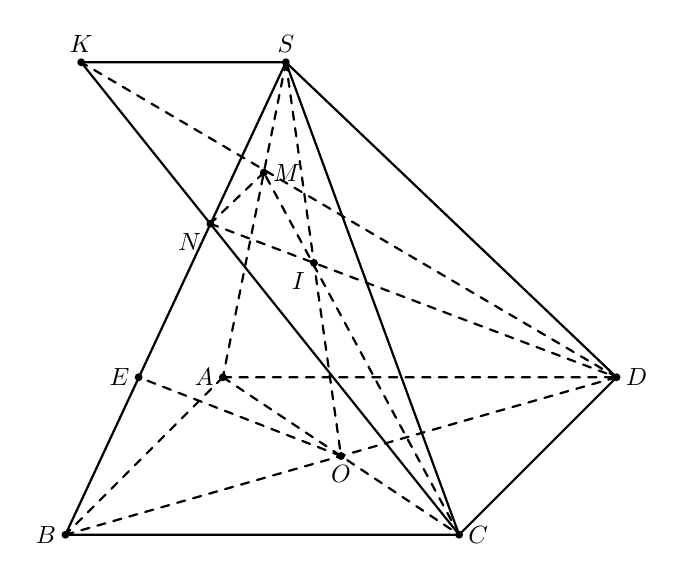
\begin{tikzpicture}[line join=round,line cap=round,>=stealth,thick]
    \coordinate  (A) at (-2,0);
    \coordinate (B) at (-4,-2); 
    \coordinate (C)  at (1,-2);
    \coordinate  (D) at (3,0);
    \coordinate (S)  at (-1.2,4);
    \coordinate (E) at (-3.07,0); 
    \coordinate (K) at  (-3.8,4);
     \coordinate (M) at (-1.48,2.6);
    \coordinate (N) at (-2.16,1.95); 
    \coordinate (O) at (intersection of A--C  and B--D);
    \coordinate  (I) at (intersection of N--D and S--O);
     \draw[dashed](S)--(A)
      (A)--(B)
      (A)--(D)
     (A)--(C) 
     (B)--(D) 
     (S)--(O) 
     (N)--(D) 
     (C)--(M) 
      (M)--(N)
     (O)--(E) 
      (D)--(K);
     \draw (S)--(B)
      (S)--(C)
     (S)--(D) 
     (B)--(C) 
      (C)--(D)
      (C)--(K)
      (S)--(K);
    \foreach \i  in {S,A,B,C,D,O,E,N,M,I,K}{\draw[fill=](\i) circle (1pt);}
    \foreach \i in {K,S}{\draw (\i) node[scale=0.9,above]{$\i$};} 
    \foreach \i in  {N,I}{\draw (\i) node[scale=0.9,below left]{$\i$};}
    \foreach \i  in {E,B,A}{\draw (\i) node[scale=0.9,left]{$\i$};}
    \foreach \i in {C,D,M}{\draw  (\i) node[scale=0.9,right]{$\i$};}
    \foreach \i  in {O}{\draw (\i) node[scale=0.9,below]{$\i$};}
   \end{tikzpicture}
 \end{center}
 \begin{itemchoice}
  \itemch \textbf{Đúng}. Trong mặt phẳng  $(SAC)$, kẻ $CI$ cắt $SA$ tại $M$.
  \itemch \textbf{sai}. Trong mặt phẳng $(SBD)$,  kẻ $DI$ cắt $SB$ tại $N$.\\
  $\text{Vì}\heva{&M  \in CI, CI \subset(ICD) \\&M \in SA} \Rightarrow M=SA \cap(ICD)$.\\
  $\text {Tương tự} \heva{&N \in  DI, DI \subset(ICD) \\ &N \in SB} \Rightarrow N=SB \cap(ICD)$.\\
  Gọi $E$ là trung điểm $BN$, $OE$ là đường trung bình của tam giác $BDN \Rightarrow  OE \parallel DN$.\\
  Trong tam giác $SOE$, ta có  $NI$ qua trung điểm $I$ của $SO$ và $NI \parallel OE$, $N$ là trung điểm của $SE$.\\
  Vậy $SN=NE=EB$ hay  $SN=\dfrac{1}{3}SB$.
  \itemch \textbf{sai}. Ta có $SM=\dfrac{1}{3}SA$.\\ 
   Khi đó hai tam giác $SMN$, $SAB$ đồng dạng vì có góc $S$ chung và $\dfrac{SM}{SA}=\dfrac{SN}{S B}=\dfrac{1}{3}$.\\
  Xét tam giác $SAB$, theo định lí Thalès, ta  có
   $$\dfrac{MN}{AB}=\dfrac{SM}{S A}=\dfrac{1}{3} \Rightarrow MN=\dfrac{AB}{3}=\dfrac{a}{3}.$$
  \itemch \textbf{Đúng}. 
  Ta có  $S$ là điểm chung của hai mặt phẳng $(SBC)$ và $(SAD)$.\\
  $\text{Ta có} \heva{&K \in CN,\, CN \subset(SBC) \\&K \in DM,\, DM  \subset(SAD)} \Rightarrow K \in(SBC) \cap(SAD)$.\\
  $\text{Vì vậy} SK=(SBC) \cap(SAD)$.\\ 
  $\text{Khi  đó} \heva{&SK=(SBC) \cap(SAD) \\ &BC \subset(SBC), AD \subset(SAD)\\ &BC \parallel AD}\Rightarrow SK \parallel BC \parallel AD$.
\end{itemchoice}}
\end{ex}

% nguồn: Ok_dungsai_lop11_Lan1
\begin{ex}%[1H4H2-3]%[ma:cde3e84d]
 Cho tứ diện $ABCD$ có $I$, $J$ theo thứ tự là trung điểm của các cạnh $BC$, $BD$. Gọi $(P)$ là mặt phẳng qua $I$, $J$ và cắt các cạnh $AC$, $AD$ lần lượt tại  hai điểm $M$, $N$. Khi đó:
  \choiceTF
  {\True $IJ \parallel CD$,  $IJ=\dfrac{1}{2} CD$}
  {$MN$  cắt $DC$}
  {\True  $IJNM$ là một hình thang}
  {\True Để $IJNM$ là hình bình  hành thì $M$ là trung điểm của đoạn $AC$}
  \loigiai{
  \begin{center}
   \begin{tikzpicture}[line join=round,line cap=round,>=stealth,scale=0.6,font=\footnotesize]
     \foreach \x/\y/\n in {0/0/B,2/-2/C,6/0/D} \coordinate (\n) at (\x,\y); 
      \coordinate (A) at ($(B)+(2,4)$);
      \coordinate (I) at ($(B)!0.5!(C)$);
     \coordinate (J) at  ($(B)!0.5!(D)$);
     \coordinate (M) at ($(A)!1/3!(C)$); 
     \coordinate (N) at  ($(A)!1/3!(D)$);
     \draw  (A)--(B)--(C)--(D)--(A)--(C)
      (I)--(M)--(N); 
     \draw[dashed]  (B)--(D)
       (N)--(J)--(I);
      \foreach \t/\g in {A/90,B/180,C/-90,D/0,I/-150,J/50,M/-180,N/45}{
      \draw[fill=black] (\t) circle (1pt) node[shift={(\g:8pt)}]{$  \t $};
      }
    \end{tikzpicture}
  \end{center}
  \begin{itemize}
   \item Ta có $IJ$ là đường trung bình của tam giác $BCD$ nên $IJ  \parallel CD$, $IJ=\dfrac{1}{2} CD$.\\
   Khi đó $\heva{&(P) \cap(ACD)=MN \\& IJ \subset(P),  CD \subset(ACD)\\& IJ \parallel CD}\Rightarrow MN \parallel IJ \parallel CD$.\\
   Vì  vậy $IJNM$ là một hình thang.
   \item Ta có $IJ \parallel MN$. Vì vậy, $IJNM$ là hình bình hành  khi và chỉ khi $IJ=MN$.\\
   Khi đó, $MN=\dfrac{1}{2}  CD$, $MN \parallel CD$.\\
   Suy ra  $MN$ là đường trung bình của tam giác $ACD$, hay $M$ là trung điểm của $AC$.
  \end{itemize}
  \begin{itemchoice}
   \itemch  Đúng.
   \itemch  Sai.
    \itemch Đúng.
   \itemch  Sai.
  \end{itemchoice}
  }
\end{ex}

% nguồn: Ok_dungsai_lop11_Lan2
\begin{ex}%[1H4H2-3]%[ma:bad432a2]
	Cho hình chóp $S.ABCD$ có $ABCD$ là tứ giác không có cạnh nào song song với nhau. Gọi $O$ là giao điểm của $AC$ và $BD$, $M$ là  điểm thuộc miền trong của tam giác $SAB$, $I$ là giao điểm của $AB$ và $CD$.
	 \choiceTF
		{Điểm $I$ là  một điểm chung của hai mặt phẳng $(SAC)$ và $(SBD)$}
		{\True Giao tuyến của hai mặt phẳng $(SAC)$ và $(SBD)$ là đường thẳng $SO$} 
		{Giao tuyến  của hai mặt phẳng $(SAB)$ và $(SCD)$ là đường thẳng $SM$}
		{Nếu $BC\parallel AD$ thì giao  tuyến của hai mặt phẳng $(MBC)$ và $(SAD)$ là đường thẳng $d$ song song với $AD$ và đi qua điểm $M$}
	 \loigiai{
		\begin{center}
			\begin{tikzpicture}[scale=1,font=\footnotesize,line join=round,line cap=round,>=stealth]
					\path  (0,0) coordinate (I)++(0:6) coordinate (B)
						(-30:6) coordinate (C) 
						($(I)!2/5!(B)$)  coordinate (A)
						($(I)!3/5!(C)$) coordinate (D) 
						(60:4) coordinate  (S)
						 (20:3.7) coordinate (M)
						(intersection of A--C  and B--D) coordinate (O)
						 (intersection of A--S and B--M) coordinate (E);
					 \draw[dashed] (I)--(B)--(M)--(C)--(A)
						(O)--(S)--(A)--(D)--(B) 
						 (M)--(E);
					\draw  (S)--(I)--(C)--(B)--cycle
						(D)--(S)--(C); 
					\foreach \diem/\vitri in  {A/-130,B/0,C/-20,D/-120,S/90,O/-110,M/75,I/170,E/170}{
						\fill  (\diem) circle (1pt)
						($(\diem)+(\vitri:2mm)$)  node[scale=.8]{$\diem$};
					 }
				\end{tikzpicture}
		\end{center}
		\begin{itemchoice}
			\itemch Sai. Xét hai  mặt phẳng $(SAC)$ và $(SBD)$.\\
			Ta có $\heva{&S\in (SAC), S\in (SBD) \\&O\in AC, AC\subset (SAC) \\&O\in BD, BD\subset (SBD)}$ nên giao tuyến của hai mặt phẳng $(SAC)$ và $(SBD)$ là  đường thẳng $SO$, mà $SO$ không đi qua điểm $I$.
			\itemch Đúng. Xét hai mặt phẳng  $(SAB)$ và $(SCD)$ có: \\
			$\heva{&S\in (SAB) \\&S\in (SCD)}$ nên  $S$ là một điểm chung của hai mặt phẳng $(SAB)$ và $(SCD)$.\\
			Mặt khác $\heva{&I\in  AB, AB\subset (SAB) \\&I\in CD, CD\subset (SCD)}$ nên $I\in (SAB)\cap (SCD)$. \\
			Vậy giao tuyến của hai  mặt phẳng $(SAB)$ và $(SCD)$ là đường thẳng $SI$.
			\itemch Sai. Nếu $BC\parallel AD$, xét hai  mặt phẳng $(MBC)$ và $(SAD)$.\\
			Trong mặt phẳng $(SAB)$  gọi $E$ là giao điểm của $BM$ và $SA$, ta có: \\
			 $\heva{&E\in BM, BM\subset (MBC) \\&E\in SA, SA\subset (SAD)}\Rightarrow E\in (MBC)\cap (SAD)$.\\
			Mặt khác, có $\heva{&BC\parallel AD \\&BC\subset (MBC) \\&AD\subset (SAD)}$ nên giao tuyến của hai mặt phẳng $(MBC)$  và $(SAD)$ là đường thẳng $d$ song song với $AD$ và đi qua điểm $E$.
		\end{itemchoice}
	 }
\end{ex}

% nguồn: Ok_dungsai_lop11_Lan2
\begin{ex}%[1H4H2-3]%[ma:56b02c40]
	Cho hình chóp $S.ABCD$ có đáy là hình thang, $AD$ là đáy lớn và $AD=2BC$. Gọi $E$ là giao điểm của  $AB$ và $CD$, $F$ là trung điểm $AD$.
	 \choiceTF
		{\True Giao tuyến của $(SAC)$ và $(SAD)$  là đường thẳng $SA$}
		{\True Giao tuyến của  $(SAB)$ và $(SCD)$ là đường thẳng $SE$}
		{Giao tuyến của $(SAD)$ và $(SBC)$ là đường thẳng $d$ đi qua $S$ và song song  cạnh $CD$}
		{Giao tuyến của $(SAB)$ và $(SFC)$ là đường thẳng $d'$ đi qua $S$ và song song cạnh  $CD$}
	 \loigiai{
		\begin{center}
			\begin{tikzpicture}[scale=1,font=\footnotesize,line join=round,line cap=round,>=stealth]
					\path  (0,0) coordinate (A)++(0:6) coordinate (D)++(-130:2) coordinate (C)++(180:3) coordinate (B)
						(80:3)  coordinate (S)
						(intersection of A--B and C--D)  coordinate (E)
						 ($(A)!.5!(D)$) coordinate (F);
					\draw[dashed] (A)--(D) 
						(F)--(C)--(A)--(B)--(C); 
					\draw  (S)--(A)--(B)--(S)--(D)--(C)
						(S)--(C)--(E)--(B) 
						 (S)--(E);
					\foreach \diem/\vitri  in {A/150,B/-110,C/-20,D/0,S/90,E/-30,F/135}{
						\fill  (\diem) circle (1pt)
						($(\diem)+(\vitri:2mm)$)  node[scale=.8]{$\diem$};
					 }
				\end{tikzpicture}
		\end{center}
		\begin{itemchoice}
			 \itemch Đúng. vì $(SAC)\cap (SAD)=SA$.
			\itemch Đúng.  Ta có $S\in (SAB)\cap (SCD)$. \hfill $(1)$ \\
			Mà $\heva{&E\in AB\subset (SAB)  \\&E\in CD\subset (SCD)} \Rightarrow E\in (SAB)\cap (SCD)$. \hfill $(2)$ \\
			Từ $(1)$ và  $(2) \Rightarrow (SAB)\cap (SCD)=SE$.
			\itemch Sai. 
			Ta có 
			$\begin{aligned}
			\heva{&S\in (SAD)\cap (SBC) \\&AD\parallel BC \\&AD\subset (SAD);BC\subset (SBC)}\Rightarrow (SAD)\cap (SBC)=d 
		\end{aligned}$
		với  $d\parallel AD$ và đi qua $S$.
		 \itemch Sai.
		Xét tứ giác $ABCF$,  ta có $\heva{&BC\parallel AF \\&BC=AF=\dfrac{AD}{2}} \Rightarrow ABCF$ là hình bình hành.\\
		 Ta có $\heva{&S\in (SAB)\cap (SCF) \\&AB\parallel FC \\&AB\subset (SAB); FC\subset (SCF)}\Rightarrow (SAB)\cap (SCF)=d'$, với $d'\parallel AB$ và đi qua $S$.
	\end{itemchoice}
} 
\end{ex}

% nguồn: Ok_dungsai_lop11_Lan2
\begin{ex}%[1H4H2-3]%[ma:5be51744]
	Cho hình chóp $S.ABCD$. Gọi $M$, $N$ là hai điểm trên cạnh $SB$, $CD$. Mặt phẳng $(P)$ qua $MN$ và song song với $SC$. Kẻ  $MK\parallel SC$ ($K\in BC$), $NP\parallel SC$ ($P\in SD$), $EH\parallel SC$ ($H\in SA$).
	 \choiceTF
		{$MK$ là giao tuyến của mặt phẳng  $(P)$ và mặt phẳng $(SCD)$}
		{$NP$ là giao tuyến của mặt phẳng  $(P)$ và mặt phẳng $(SBC)$}
		{\True $EH$  là giao tuyến của mặt phẳng $(P)$ và mặt phẳng $(SAC)$}
		{\True Thiết diện của $(P)$ với hình chóp  $S.ABCD$ là ngũ giác $MKNPH$}
	 \loigiai{
		\begin{center}
			\begin{tikzpicture}[scale=1,font=\footnotesize,line join=round,line cap=round,>=stealth]
					\coordinate[label=left:$A$] (A)  at (0,0);
					\coordinate[label=below left:$B$] (B)  at (-60:3);
					\coordinate[label=below right:$C$] (C) at (-35:5); 
					\coordinate[label=right:$D$]  (D) at (4,0);
					\coordinate[label=above:$S$]  (S) at (80:3);
					\coordinate[label=left:$M$] (M)  at ($(S)!.4!(B)$);
					\coordinate[label=right:$N$] (N)  at ($(D)!.2!(C)$);
					\coordinate[label=below:$K$] (K) at ($(C)!.4!(B)$); 
					\coordinate[label=right:$P$] (P) at  ($(D)!.2!(S)$);
					\coordinate[label=left:$H$]  (H) at ($(S)!.2!(A)$);
					\coordinate[label=below:$E$] (E)  at ($(C)!.2!(A)$);
					\path[pattern = north  east lines] (M)--(H)--(P)--(N)--(K)--cycle;
					\draw (A)--(B)--(C)--(D)--(S)--cycle  (B)--(S)--(C)
						(H)--(M)--(K) 
						(N)--(P); 
					 \draw[dashed] (C)--(A)--(D)
						 (E)--(H)--(P)
						 (N)--(K);
					\foreach \diem in {A,B,C,D,S,M,N,K,P,E,H} \fill  (\diem) circle (1pt);
				\end{tikzpicture}
		\end{center}
		\begin{itemchoice}
			\itemch  Mặt phẳng $(SBC)$ chứa đường thẳng $SC$ song song với mặt phẳng $(P)$ nên mặt phẳng $(SBC)$ cắt $(P)$ theo giao tuyến song song với $SC$.\\
			 Kẻ $MK\parallel SC$ ($K\in BC$).\\
			Khi đó $MK$ là giao tuyến  của hai mặt phẳng $(P)$ và $(SBC)$.
			\itemch Mặt phẳng $(SCD)$  chứa đường thẳng $SC$ song song với mặt phẳng $(P)$ nên mặt phẳng $(SCD)$ cắt $(P)$ theo giao tuyến song song với $SC$.\\
			Kẻ $NP\parallel SC$ ($P\in  SD$).\\
			Khi đó $NP$ là giao tuyến của hai mặt phẳng $(P)$ và $(SCD)$. 
			\itemch Mặt phẳng $(SAC)$ chứa đường thẳng $SC$ song song với $(P)$ nên hai mặt  phẳng cắt nhau theo giao tuyến song song với $SC$.\\
			Kẻ  $EH\parallel SC$ ($H\in SA$).\\
			Khi đó $EH$ là giao  tuyến của hai mặt phẳng $(P)$ và $(SAC)$.
			\itemch Ta có $\heva{ 
			 &(SAD)\cap (P)=PM\\
			 &(SAB)\cap (P)=HM.
			 }$\\
			Vậy thiết diện của $(P)$ với hình  chóp $S.ABCD$ là ngũ giác $MKNPH$.
		\end{itemchoice}
	} 
\end{ex}

% nguồn: Ok_dungsai_lop11_Lan2
\begin{ex}%[1H4H2-3]%[ma:edc66d5a]
	Cho hình chóp $S.ABCD$ có đáy là hình bình hành. Điểm $M$ thuộc cạnh $SA$, điểm $E$ và $F$ lần lượt là trung điểm của $AB$ và  $BC$.
	\choiceTF 
		{\True $EF\parallel  AC$}
		{Giao tuyến của hai mặt phẳng $(SAB)$ và $(SCD)$ là đường thẳng qua $S$ và song song với  $AC$}
		{\True Giao tuyến của hai mặt phẳng $(MBC)$  và $(SAD)$ là đường thẳng qua $M$ và song song với $BC$}
		{\True Giao tuyến của hai mặt phẳng $(MEF)$ và $(SAC)$ là đường thẳng qua  $M$ và song song với $AC$}
	\loigiai{ 
		\begin{center}
			\begin{tikzpicture}[scale=1,font=\footnotesize,line join=round,line cap=round,>=stealth]
					\coordinate[label=below left:$A$] (A) at (0,0); 
					 \coordinate[label=below:$D$] (D) at (-50:3);
					\coordinate[label=right:$B$] (B) at (4,0); 
					\coordinate[label=right:$C$] (C)  at ($(B)-(A)+(D)$);
					\coordinate[label=below:$O$] (O) at  ($(A)!.5!(C)$);
					\coordinate[label=above:$S$] (S) at  ($(O)+(90:4)$);
					\coordinate[label=below:$E$] (E)  at ($(B)!.5!(A)$);
					\coordinate[label=below:$F$] (F)  at ($(B)!.5!(C)$);
					\coordinate[label=left:$M$]  (M) at ($(S)!0.2!(A)$);
					 \coordinate (H) at ($(B)-(A)+(S)$);
					\coordinate (G)  at ($(A)-(D)+(M)$);
					\coordinate  (K) at ($(F)-(E)+(M)$);
					 \draw (A)--(D)--(C)--(S)--cycle (S)--(D);
					\draw[dashed] (D)--(B)--(A)--(O) 
						 (S)--(O)--(C)--(B)--cycle (M)--(E)--(F)-- cycle;
					 \draw[shorten <=-1cm] (S)--(H) node[pos=0.9,sloped,above]{$x$};
					\draw[shorten <=-0.8cm,shorten >=1cm] (M)--(G)  node[pos=0.7,sloped,above]{$y$};
					 \draw[shorten <=-0.8cm] (M)--(K) node[pos=0.7,sloped,above]{$z$};
					\foreach \diem in {A,D,C,B,O,S,E,F,M} \fill (\diem)  circle (1pt);
				\end{tikzpicture}
		\end{center}
		\begin{itemchoice}
			\itemch Ta có $E$, $F$ lần lượt  là trung điểm của $AB$ và $BC$ nên $EF$ là đường trung bình của tam giác $ABC$.\\
			Do đó $EF\parallel AC$. 
			 \itemch Ta có
			 \[\heva{&S\in(SAB)\cap(SCD)\\
			&AB\subset(SAB); CD\subset(SCD)\\ 
			&AB\parallel CD. 
			 }\]
			Suy ra $Sx=(SAB)\cap(SCD)$, với $Sx$ là đường  thẳng qua $S$ và $Sx\parallel AB\parallel CD$.\\
			Do đó không thể kết  luận $Sx\parallel AC$.
			\itemch  Ta có
			 \[\heva{
			&M\in  SA, SA\subset(SAD)\\
			 &M\in(MBC).
			}\] 
			Suy ra  $M\in(MBC)\cap(SAD)$.\\
			Khi đó,  ta có
			 \[\heva{
			&BC\subset(MBC)\\ 
			 &AD\subset(SAD)\\
			&BC\parallel AD. 
			 }\]
			Suy ra $My=(MBC)\cap(SAD)$ là đường thẳng qua $M$ và  $My\parallel BC\parallel AD$.
			\itemch Ta có 
			\[\heva{ 
			&M\in SA,  SA\subset(SAC)\\
			 &M\in(MEF).
			}\] 
			Suy ra $M\in(MEF)\cap(SAC)$.\\ 
			Xét tam giác $ABC$ có $E$, $F$ lần lượt là trung điểm của $AB$  và $BC$ nên $EF$ là đường trung bình.\\
			 Suy ra $EF\parallel AC$.\\
			Khi đó, ta  có
			\[\heva{ 
			 &EF\subset(MEF)\\
			 &AC\subset(SAC)\\
			 &EF\parallel AC.
			 }\]
			Suy ra $Mt=(MEF)\cap(SAC)$ là đường thẳng qua $M$ và  $Mt\parallel EF\parallel AC$.
		\end{itemchoice}
	} 
\end{ex}

% nguồn: Ok_dungsai_lop11_Lan2
\begin{ex}%[1H4H2-3]%[ma:93e53c26]
	Cho hình chóp $S.ABCD$ có đáy $ABCD$ là hình bình hành. Gọi $M$, $N$, $P$ lần lượt là trung điểm của $SB$, $AB$, $CD$. Gọi $d$ là giao tuyến của hai mặt phẳng $(MNP)$ và $(SBC)$. Xét tính đúng sai của các mệnh đề sau 
	\choiceTF 
		{\True $d$ đi qua trung điểm  của $SC$}
		{\True $d\parallel  AD$}
		{$d$ cắt $NP$} 
		{\True $d\parallel  BC$}
	\loigiai{ 
	 \immini{
		\begin{itemchoice}
			\itemch Đúng. Ta có $\heva{&(MNP)\cap (SBC)=d\\  &(MNP)\cap (ABCD)=NP\\ &(ABCD)\cap (SBC)=BC \\ &AB\parallel CD}$\\
			$\Rightarrow d=MQ\parallel BC \parallel  NP$.
			\itemch Đúng. Vì $d=MQ\parallel  BC\parallel AD$.
			 \itemch Sai. Vì $d\parallel NP$.
			\itemch Đúng. Vì $d=MQ\parallel BC\parallel  AD$.
		\end{itemchoice}
		 }
		{ 
		\begin{tikzpicture}[scale=1,font=\footnotesize,line join=round,line cap=round,>=stealth]
				\path (0,0) coordinate (A)++(0:3) coordinate (B)++(-150:2) coordinate (C) 
					($(A)-(B)+(C)$)  coordinate (D)
					 (80:3) coordinate (S)++(0:2) coordinate (p)
					(intersection  of A--C and B--D) coordinate (O)
					 ($(S)!.5!(B)$) coordinate (M)
					($(A)!.5!(B)$) coordinate (N) 
					($(C)!.5!(D)$)  coordinate (P)
					($(S)!.5!(C)$) coordinate (Q); 
				 \draw[dashed] (S)--(A)--(B)
					 (A)--(D)
					 (M)--(N)--(P)--cycle;
				\draw (B)--(C)--(D)--(S)--cycle  (S)--(C)
					 (M)--(Q)--(P);
				\foreach \diem/\vitri in {A/160,B/20,C/-20,D/200,S/90,O/-100,M/10,N/40,P/-90,Q/180}{ 
					\fill (\diem) circle  (1pt)
					($(\diem)+(\vitri:2mm)$) node[scale=.8]{$\diem$}; 
				 }
			\end{tikzpicture}
		} 
	} 
\end{ex}

% nguồn: Ok_dungsai_lop11_Lan2
\begin{ex}%[1H4H2-3]%[ma:52ba52fc]
	Cho tứ diện $ABCD$. Gọi $I$ và $J$ lần lượt  là trung điểm của $AD$ và $AC$, $G$ là trọng tâm của tam giác $BCD$.
	\choiceTF 
		{\True $IJ\parallel CD$} 
		{Giao  tuyến của hai mặt phẳng $(GIJ)$ và $(BCD)$ là đường thẳng qua $G$ và song song với $BC$}
		{Cho biết $CD=6$. Biết  $(GIJ)$ cắt $BC$, $BD$ lần lượt tại $M$ và $N$. Khi đó $2IJ+3MN=17$}
		{Cho biết $CD=6$.  Biết $(GIJ)$ cắt $BC$, $BD$ lần lượt tại $M$ và $N$. Khi đó $3IJ+2MN=18$}
	 \loigiai{
		\begin{center}
			\begin{tikzpicture}[scale=1,font=\footnotesize,line join=round,line cap=round,>=stealth]
					\coordinate[label=left:$B$] (B) at  (0,0);
					\coordinate[label=right:$D$] (D)  at (4,0);
					\coordinate[label=below  left:$C$] (C) at (-40:3.5);
					\coordinate[label=above:$A$] (A) at (30:4); 
					\coordinate[label= right:$I$] (I) at  ($(A)!.5!(D)$);
					\coordinate[label=below right:$J$]  (J) at ($(A)!.5!(C)$);
					\coordinate[label=below:$E$] (E) at ($(D)!.5!(C)$); 
					\coordinate[label=below:$M$]  (M) at ($(B)!2/3!(C)$);
					\coordinate[label=above:$N$] (N) at  ($(B)!2/3!(D)$);
					\coordinate[label=above left:$G$] (G) at (intersection of  B--E and M--N);
					 \draw (B)--(C)--(D)--(A)--cycle (A)--(C)
						 (I)--(J);
					\draw[dashed]  (E)--(B)--(D)
						(M)--(N); 
					\foreach \diem in {B,C,D,A,I,J,E,M,N,G} \fill  (\diem) circle (1pt);
				\end{tikzpicture}
		\end{center}
		\begin{itemchoice}
			 \itemch Ta có $IJ$ là đường trung bình của tam giác $ACD$ nên $IJ\parallel CD$.
			\itemch Ta  xét giao tuyến của hai mặt phẳng $(GIJ)$ và $(BCD)$\\
			Vì $IJ$ là đường trung  bình tam giác $ACD$ nên $IJ\parallel CD$.\\
			Ta  có
			 \[\heva{
			 &G\in(GIJ)\cap(BCD)\\
			&IJ\parallel CD\\ 
			&IJ\subset(GIJ), CD\subset(BCD). 
			 }\]
			Suy ra $Gx=(GIJ)\cap(BCD)$ là đường thẳng qua $G$ và  $Gx\parallel IJ\parallel CD$.\\
			Do đó không thể kết luận $Gx\parallel BC$. 
			\itemch Trong mặt phẳng $(BCD)$, kẻ $Gx$ song song $CD$  cắt $BC$ tại $M$, cắt $BD$ tại $N$.\\
			Gọi $E$ là trung  điểm $CD$.Theo định lý Thales, ta có
			 \[\dfrac{MN}{CD}=\dfrac{BM}{BC}=\dfrac{BG}{BE}=\dfrac{2}{3}.\]
			Suy  ra $\dfrac{MN}{6}=\dfrac{2}{3}\Rightarrow MN=4$.\\
			Mặt khác, ta cũng  có
			 \[IJ=\dfrac{1}{2}CD=\dfrac{1}{2}\cdot 6=3.\]
			 Suy ra
			 $2IJ+3MN=2\cdot 3+3\cdot 4=6+12=18\ne 17$.
			\itemch Ta có  $IJ=3$, $MN=4$ nên
			\[3IJ+2MN=3\cdot 3+2\cdot 4=9+8=17.\] 
		\end{itemchoice}
	 }
\end{ex}

% nguồn: Ok_dungsai_lop11_Lan2
\begin{ex}%[1H4H2-3]%[ma:dc5d7c01]
	Cho hình chóp $S.ABCD$ có đáy $ABCD$ là hình bình hành. Gọi $d$ là giao tuyến của hai mặt  phẳng $(SAB)$ và $(SCD)$. Xét tính đúng sai của các mệnh đề sau
	 \choiceTF
		 {\True $d$ đi qua điểm $S$}
		 {\True $d\parallel CD$}
		 {$d\parallel AD$}
		{\True $d\parallel  AB$}
	 \loigiai{
	\immini{ 
		Ta có $S\in (SAB)\cap  (SCD)$, $AB\parallel CD$.\\
		Suy ra $(SAB)\cap (SCD)=d$  với $S\in d$ và $d\parallel AB$, $d\parallel CD$.
		\begin{itemchoice}
			\itemch Đúng. Do $S\in (SAB)\cap (SCD) \Rightarrow  S\in d$.
			\itemch Đúng. Do $\heva{&AB\parallel CD \\& AB\subset (SAB)\\ &CD\subset (SCD)} \Rightarrow d\parallel AB\parallel  CD$.
			\itemch Sai. Do $d\parallel AB\parallel CD\Rightarrow d\nparallel AD$. 
			 \itemch Đúng. Do $\heva{&AB\parallel CD \\& AB\subset (SAB)\\ &CD\subset (SCD)} \Rightarrow d\parallel AB\parallel CD$.
		\end{itemchoice}
		 }
		{ 
		\begin{tikzpicture}[scale=1,font=\footnotesize,line join=round,line cap=round,>=stealth]
				\path (0,0) coordinate  (A)++(0:3) coordinate (B)++(-140:1.5) coordinate (C)
					($(A)-(B)+(C)$) coordinate  (D)
					(80:3) coordinate (S)++(0:2)  coordinate (p)
					(intersection  of A--C and B--D) coordinate (O);
				 \draw[dashed] (S)--(A)--(B)
					(A)--(D); 
				\draw (B)--(C)--(D)--(S)--cycle  (S)--(C);
				 \draw ($(S)+(180:.2)$) -- ($(p)+(180:.2)$) node[above]{$d$};
				\foreach  \diem/\vitri in {A/160,B/20,C/-20,D/200,S/90,O/-90}{
					\fill  (\diem) circle (1pt)
					 ($(\diem)+(\vitri:2mm)$) node[scale=.8]{$\diem$};
				 }
			\end{tikzpicture}
		 }
	 }
\end{ex}

% nguồn: Ok_dungsai_lop11_Lan1
\begin{ex}%[1H4V2-3]%[ma:49d66aa9]
 Cho tứ diện $ABCD$, gọi $I$ và $J$ lần lượt là trung điểm của $AD$ và $AC$, $G$ là trọng  tâm của tam giác $BCD$.
 \choiceTF 
  {\True $IJ \parallel  CD$}
  {Giao tuyến của hai mặt phẳng $(GIJ)$ và $(BCD)$ là  đường thẳng qua $G$ và song song với $BC$}
  {Cho biết $CD=6$. Biết $(GIJ)$  cắt $BC$, $BD$ lần lượt tại $M$ và $N$. Khi đó $2IJ+3MN=17$}
  {Cho biết $CD=6$. Biết $(GIJ)$ cắt  $BC$, $BD$ lần lượt tại $M$ và $N$. Khi đó $3IJ+2MN=18$}
  \loigiai{
  \begin{center}
   \begin{tikzpicture}[line join=round,line cap=round,>=stealth,scale=0.6,font=\footnotesize]
     \foreach \x/\y/\n  in {0/0/B,2/-2/C,6/0/D} \coordinate (\n) at (\x,\y);
     \coordinate (A) at  ($(B)+(2,4)$);
     \coordinate (I) at ($(A)!0.5!(D)$); 
     \coordinate (J) at ($(A)!0.5!(C)$); 
     \coordinate (E) at ($(D)!0.5!(C)$); 
     \coordinate (G) at  ($(B)!2/3!(E)$);
     \coordinate (M) at  ($(B)!2/3!(C)$);
     \coordinate (N) at  ($(B)!2/3!(D)$);
     \draw  (A)--(B)--(C)--(D)--(A)--(C)
       (I)--(J);
     \draw[dashed]  (B)--(D)
      (M)--(N) 
      (B)--(E); 
     \foreach \t/\g  in {A/90,B/180,C/-90,D/0,J/210,I/30,M/-150,N/45,G/-90,E/-30}{
      \draw[fill=black] (\t)  circle (1pt) node[shift={(\g:8pt)}]{$ \t $};
     } 
    \end{tikzpicture}
  \end{center}
  \begin{itemize}
   \item Ta có $IJ$ là đường trung bình của $\triangle ACD$ nên $IJ\parallel CD$. 
   \item Ta có $\heva{&G \in(GIJ) \cap(BCD) \\& IJ \parallel CD \\& IJ \subset(GIJ),  CD \subset(BCD)}$ \\
   $\Rightarrow  Gx=(GIJ) \cap(BCD)$, trong đó $Gx$ là đường thẳng qua $G$ và $Gx \parallel IJ \parallel CD$.
   \item Trong mặt phẳng $(BCD)$, kẻ $Gx$ song song  $CD$ cắt $BC$ tại $M$, cắt $BD$ tại $N$.\\
   Gọi $E$ là trung điểm $CD$,  theo định lí Thalès, ta có
   \begin{center}
    $\dfrac{BM}{BC}=\dfrac{BG}{BE}=\dfrac{2}{3}$ (vì $GM\parallel CE$); $\dfrac{MN}{CD}=\dfrac{BM}{BC}$ (vì $MN\parallel CD$). 
   \end{center}
    Suy ra $\dfrac{MN}{CD}=\dfrac{2}{3}$ hay $MN=\dfrac{2}{3}CD=\dfrac{2}{3} \cdot 6=4$.\\
   Vì $IJ$ là đường trung bình tam giác $ACD$ nên $IJ=\dfrac{1}{2}  CD=\dfrac{1}{2} \cdot 6=3$.\\
   Do đó $2IJ+3MN=2 \cdot 3+3 \cdot 4=18$  và $3IJ+2MN=3\cdot 3+2\cdot 4=17$.
  \end{itemize}
  \begin{itemchoice}
   \itemch Đúng. 
    \itemch Sai.
   \itemch Sai. 
    \itemch Sai.
  \end{itemchoice}
 } 
\end{ex}

% nguồn: Ok_dungsai_lop11_Lan2
\begin{ex}%[1H4V2-3]%[ma:6e93b626]
	Cho hình chóp $S.ABCD$, có đáy $ABCD$ là một hình bình hành tâm $O$.  Gọi $I$, $K$ lần lượt là trung điểm của $SB$ và $SD$.
	 \choiceTF
		{\True $SO$ là giao tuyến của hai mặt phẳng $(SAC)$ và $(SBD)$} 
		{Giao điểm $J$ của $SA$ với mặt phẳng $(CKB)$  thuộc đường thẳng đi qua $K$ và song song với $DC$}
		{\True Giao  tuyến của hai mặt phẳng $(OIA)$ và $(SCD)$ là đường thẳng đi qua $C$ và song song với $SD$}
		 {\True $CD\parallel IJ$}
	 \loigiai{
		\begin{center}
			\begin{tikzpicture}[scale=1,font=\footnotesize,line join=round,line cap=round,>=stealth]
					 \coordinate[label=below left:$A$] (A) at (0,0);
					\coordinate[label=below:$D$]  (D) at (-50:3);
					\coordinate[label=right:$B$] (B)  at (4,0);
					\coordinate[label=right:$C$] (C) at  ($(B)-(A)+(D)$);
					\coordinate[label=below:$O$] (O) at  ($(A)!.5!(C)$);
					\coordinate[label=above:$S$] (S) at  ($(O)+(90:4)$);
					 \coordinate[label=left:$I$] (I) at ($(B)!.5!(S)$);
					\coordinate[label=left:$K$] (K) at ($(S)!.5!(D)$); 
					 \coordinate (H) at ($(A)-(D)+(K)$);
					\coordinate (G) at  ($(I)-(O)+(C)$);
					\draw  (A)--(D)--(C)--(S)--cycle (S)--(D);
					\draw[dashed]  (D)--(B)--(A)--(O)
						(S)--(O)--(C)--(B)--cycle  (B)--(K)--(C)
						(O)--(I); 
					\draw[shorten <=-2cm] (K)--(H)  node[pos=0.9,sloped,above]{$x$};
					\draw[shorten <=-0.5cm] (C)--(G) node[pos=0.9,sloped,above]{$y$}; 
					\foreach  \diem in {A,D,C,B,O,S,I,K} \fill (\diem) circle (1pt);
				\end{tikzpicture}
		\end{center}
		\begin{itemchoice}
			\itemch  Ta có
			 $\heva{
			&O\in AC\subset(SAC)\\ 
			&O\in  BD\subset(SBD).
			}$\\ 
			Suy ra $O\in(SAC)\cap(SBD)$.\\ 
			Mặt  khác $S\in (SAC)\cap(SBD)$ nên $SO=(SAC)\cap(SBD)$.
			\itemch Tứ giác $ABCD$ là hình bình hành nên $AB\parallel CD$ và  $AD\parallel BC$.\\
			Ta có 
			 $\heva{
			&AD\subset(SAD)\\ 
			 &BC\subset(SBC)\\
			 &Kx=(KBC)\cap(SAD).
			}$\\ 
			Suy ra $Kx\parallel AD\parallel  BC$.\\
			 Trong mặt phẳng $(SAD)$, gọi $J=Kx\cap SA$. Ta có
			$\heva{ 
			 &J\in SA\\
			 &J\in Kx\subset(BKC).
			}$\\ 
			 Suy ra $J=SA\cap(BKC)$.\\
			Vậy không thể kết luận $J$ thuộc đường  thẳng qua $K$ và song song $DC$.
			\itemch Ta có $OI$ là đường trung bình  của $\triangle SBD$.\\
			Suy ra $OI\parallel  SD$.\\
			Khi  đó, ta có
			 \[\heva{
			&OI\parallel  SD\\
			 &OI\subset(OIA)\\
			 &SD\subset(SCD)\\
			&C\in(OIA)\cap(SCD) 
			}\] 
			Suy ra $Cy=(OIA)\cap(SCD)$ và $Cy\parallel SD\parallel OI$. 
			\itemch Ta có $IJ$ là đường trung bình của tam  giác $\triangle SAB$.\\
			Suy  ra $IJ\parallel AB$.\\
			Mặt khác, ta có  $AB\parallel CD$ (do $ABCD$ là hình bình hành).\\
			 Suy ra $CD\parallel IJ$.
		\end{itemchoice}
	 }
\end{ex}

% nguồn: Ok_dungsai_lop11_Lan2
\begin{ex}%[1H4V2-3]%[ma:d3efa129]
	Cho hình chóp $S.ABCD$ có đáy $ABCD$ là hình bình hành. Gọi $E$, $F$ lần lượt là trung điểm của $AB$ và $BC$, gọi $M$ là điểm nằm trên cạnh $SA$. Gọi $d_1$, $d_2$, $d_3$ lần lượt  là giao tuyến của các cặp mặt phẳng $(SAB)$ và $(SCD)$, $(MBC)$ và $(SAD)$, $(MEF)$ và $(SAC)$.
	\choiceTF 
		 {\True $EF \parallel AC$}
		{$d_1$ đi qua điểm $S$ và song song với $AC$} 
		 {\True $d_2$ đi qua điểm $M$ và song song với $BC$}
		{\True $d_3$ đi qua điểm $M$ và  song song với $AC$}
	 \loigiai{
		\begin{center}
			\begin{tikzpicture}[scale=0.8,font=\footnotesize,line join=round,line cap=round,>=stealth]
					\def\a{4} 
					 \def\b{0.4}
					\coordinate (B) at  (0,0);
					\coordinate  (C) at (\a*1.2,0);
					\coordinate (A) at  ($(B)+(\a*0.6,\a*0.5)$);
					\coordinate (D) at ($(A)+(C)-(B)$); 
					 \coordinate (S) at ($(\a*0.8,\a*1.7)$);
					\coordinate (E) at ($(A)!0.5!(B)$); 
					\coordinate (F)  at ($(B)!0.5!(C)$);
					 \coordinate (M) at ($(S)!\b!(A)$);
					\coordinate (M1) at ($(S)!\b!(C)$); 
					\coordinate (t)  at ($(M)!1.5!(M1)$);
					\coordinate  (z) at ($(B)+(S)-(A)$);
					\coordinate (t)  at ($(M)!2.2!(M1)$);
					 \coordinate (M3) at ($(S)!\b!(D)$);
					\coordinate (y)  at ($(M)!2.2!(M3)$);
					 \draw (S)--(B)--(C)--(D)--(S)--(C)
						 (M1)--(t)
						(S)--(z) 
						(M3)--(y); 
					\draw[dashed]  (B)--(A)--(D)
						(C)--(A)--(S) 
						(C)--(M)--(E)--(F)--(M) 
						(B)--(M)--(M1) 
						(M)--(M3); 
					 \foreach \x/\label/\g in {E/\(E\)/-100,S/\(S\)/90,B/\(B\)/-90,C/\(C\)/-90,D/\(D\)/-60,A/\(A\)/140,F/\(F\)/-90,M/\(M\)/150}
					\fill (\x) circle  (1pt)
						($(\x)+(\g:3mm)$) node{\small $\x$}; 
					 \node[above] at (y) {\(y\)};
					\node[above] at (z) {\(z\)}; 
					\node[above] at (t) {\(t\)}; 
				\end{tikzpicture}
		\end{center}
		\begin{itemchoice}
			 \itemch \textbf{Đúng} \\
			Ta có  $EF$ là đường trung bình của tam giác $ABC$ nên $EF \parallel AC$.
			\itemch \textbf{Sai} \\ 
			 Ta có
			 \[
			\heva{&S \in (SAB) \cap (SCD) \\ &AB \subset  (SAB) \\&CD \subset (SCD) \\&AB \parallel CD}
			 \]
			Suy ra $(SAB) \cap (SCD)= Sz$, với $Sz \parallel AB  \parallel CD$.
			\itemch \textbf{Đúng}\\ 
			Ta  có
			 \[
			\heva{&M \in SA, SA \subset (SAD) \\ &M \in (MBC)} 
			 \Rightarrow M \in (MBC) \cap (SAD).
			 \]
			Khi  đó
			 \[
			 \heva{&M \in (MBC) \cap (SAD)\\ &BC \subset (MBC) \\ &AD \subset (SAD) \\ &BC \parallel AD}
			 \]
			Suy ra $(MBC) \cap (SAD)=My$, với $My \parallel BC \parallel AD$. 
			\itemch \textbf{Đúng} \\ 
			Ta  có
			\[ 
			\heva{&M \in  SA, SA \subset (SAC) \\ &M \in (MEF)}
			 \Rightarrow M \in (MEF) \cap (SAC).
			 \]
			Tam giác  $ABC$ có $EF$ là đường trung bình nên $EF \parallel AC$.
			 Ta có
			 \[
			\heva{&M \in (MEF) \cap (SAC)\\ &EF \subset (MEF) \\ &AC \subset (SAC)  \\&EF \parallel AC}
			\] 
			Suy ra $(MEF) \cap (SAC)=Mt$, với $Mt \parallel EF \parallel  AC$.
		\end{itemchoice}
	} 
\end{ex}

% nguồn: Ok_dungsai_lop11_Lan2
\begin{ex}%[1H4V2-3]%[ma:03035cc2]
	Cho hình chóp $S.ABCD$, có đáy $ABCD$ là  một hình bình hành tâm $O$. Gọi $I, K$ lần lượt là trung điểm của $SB$ và $SD$.
	\choiceTF 
		{\True $SO$ là giao  tuyến của $(SAC)$ và $(SBD)$}
		{Giao điểm $J$ của $SA$ với $(CKB)$ thuộc đường thẳng đi qua $K$ và song song  với $DC$}
		{\True Giao tuyến của $(OIA)$ và $(SCD)$  là đường thẳng đi qua $C$ và song song với $SD$}
		{\True  $CD \parallel IJ$}
	\loigiai{ 
		\begin{center}
			\begin{tikzpicture}[scale=0.8,font=\footnotesize,line join=round,line cap=round,>=stealth]
					\def\a{4} 
					 \def\b{0.4}
					\coordinate (B) at (0,0); 
					\coordinate (C)  at (\a*1.2,0);
					\coordinate (A)  at ($(B)+(\a*0.4,\a*0.5)$);
					\coordinate  (D) at ($(A)+(C)-(B)$);
					\coordinate (S) at ($(\a*0.5,\a*1.7)$); 
					\coordinate (O) at ($(A)!0.5!(C)$); 
					\coordinate (I)  at ($(S)!0.5!(B)$);
					\coordinate (J) at ($(S)!0.5!(A)$); 
					\coordinate (K) at ($(S)!0.5!(D)$); 
					 \coordinate (x) at ($(K)!-0.5!(J)$);
					\coordinate (y) at  ($(C)+(S)-(D)$);
					\draw (S)--(B)--(C)--(D)--(S)--(C)--(I) 
						(x)--(K)--(C)--(y); 
					\draw[dashed]  (A)--(B)--(D)--(A)--(C)
						(I)--(J)--(K)--(B) 
						(S)--(O)--(I)--(A)--cycle; 
					 \foreach \h/\label/\g in {S/\(S\)/90,B/\(B\)/-90,C/\(C\)/-90,D/\(D\)/-60,A/\(A\)/180,O/\(O\)/-100,I/\(I\)/180,J/\(J\)/160,K/\(K\)/60}
					\fill (\h)  circle (1pt)
						($(\h)+(\g:3mm)$) node{\small $\h$}; 
					\node[above] at (y)  {\(y\)};
					\node[above] at (x) {\(x\)}; 
				\end{tikzpicture}
		\end{center}
		\begin{itemchoice}
			\itemch  \textbf{Đúng} \\
			 Ta có
			 \[
			\heva{&O  \in AC, AC \subset (SAC) \\ &O \in BD, BD \subset (SBD)}
			\Rightarrow O \in  (SAB) \cap (SCD).
			\] 
			Ta  có
			\[ 
			\heva{&O  \in (SAB) \cap (SCD)\\&S \in (SAB) \cap (SCD)}
			\Rightarrow SO = (SAC)  \cap (SBD).
			 \]
			\itemch  \textbf{Sai} \\
			Tứ  giác $ABCD$ là hình bình hành nên $AB \parallel CD$ và $AD \parallel BC$.
			\[ 
			\heva{&K \in (KBC) \cap  (SAD) \\&AD \subset (SAD) \\ &BC \subset (SBC) \\&AD \parallel BC}
			 \Rightarrow
			(KBC) \cap (SAD)=Kx, Kx  \parallel AD.
			 \]
			Trong $(SAD)$ gọi $J = Kx  \cap SA$, ta có
			 \[
			\heva{ 
			&J \in SA \\ 
			 &J \in Kx, Kx \subset (BKC)}
			\Rightarrow J =  SA \cap (BKC).
			\] 
			\itemch  \textbf{Sai}\\
			Có  $OI$ là đường trung bình của $\triangle SBD \Rightarrow OI \parallel SD$.
			 \[
			\text{Ta có: } 
			\heva{&C \in  (OIA) \cap (SCD) \\&OI \parallel SD \\ &OI \subset (OIA) \\&SD \subset (SCD)}
			\Rightarrow 
			 (OIA) \cap (SCD)=Cy, Cy \parallel SD.
			 \]
			\itemch  \textbf{Sai} \\
			 Ta có $IJ$ là đường trung bình của $\triangle SAB$ nên $IJ \parallel AB$. \hfill (1)\\
			Ta có tứ giác $ABCD$  là hình bình hành nên $AB \parallel CD$. \hfill (2)\\
			Từ (1) và (2) $\Rightarrow  CD \parallel IJ$.
		\end{itemchoice}
	 }
\end{ex}

% nguồn: Ok_dungsai_lop11_Lan2
\begin{ex}%[1H4V2-3]%[ma:4a62f417]
	Cho hình chóp $S.ABCD$ có đáy $ABCD$ là hình bình  hành. Gọi $M$, $N$ lần lượt là hai điểm nằm trên các cạnh $SC$ và $SB$.
	 \choiceTF
		{\True Giao tuyến của $(SAB)$ và $(SCD)$ là đường thẳng đi qua  $S$ và song song với $AB$}
		{Giao tuyến của $(SAD)$ và $(SBC)$ là đường  thẳng đi qua $S$ và song song với $AB$}
		{\True Giao tuyến của $(ABM)$ và $(SCD)$ là đường thẳng đi qua $M$ và song song với  $AB$}
		{\True Giao tuyến của $(SAB)$ và $(NCD)$ là đường  thẳng đi qua $N$ và song song với $AB$}
	 \loigiai{
		\begin{center}
			\begin{tikzpicture}[scale=0.8,font=\footnotesize,line join=round,line cap=round,>=stealth]
					 \def\a{4}
					\coordinate  (D) at (0,0);
					 \coordinate (C) at (\a*1.2,0);
					 \coordinate (A) at ($(D)+(\a*0.5,\a*0.5)$);
					\coordinate  (B) at ($(A)+(C)-(D)$);
					\coordinate (S) at  ($(\a*0.75,\a*1.7)$);
					\coordinate (M) at  ($(S)!0.6!(C)$);
					\coordinate (N) at ($(S)!0.35!(B)$); 
					\coordinate (y)  at ($(D)+(S)-(A)$);
					\coordinate  (x) at ($(S)+(\a*0.6,0)$);
					\coordinate (z) at  ($(N)+(\a*0.5,0)$);
					 \coordinate (z1) at ($(N)+(-\a*0.3,0)$); \coordinate (t) at ($(M)+(-\a*0.8,0)$);
					 \draw (S)--(B)--(C)--(D)--(S)--(C)
						(B)--(M)--(t) 
						 (z)--(N)--(C)
						 (x)--(S)--(y);
					\draw[dashed]  (S)--(A)--(D)--(N)
						 (M)--(A)--(B)
						 (N)--(z1);
					\foreach  \h/\label/\g in {D/\(D\)/-60,A/\(A\)/-90,B/\(B\)/-90,C/\(C\)/-90,S/\(S\)/90,M/\(M\)/-120,N/\(N\)/60}
					\fill (\h) circle (1pt) 
						($(\h)+(\g:3mm)$)  node{\small $\h$};
					\node[above]  at (y) {\(y\)};
					\node[above]  at (z) {\(z\)};
					\node[above] at (t) {\(t\)}; 
					\node[above]  at (x) {\(x\)};
				\end{tikzpicture}
		\end{center}
		\begin{itemchoice}
			\itemch \textbf{Đúng}  \\
			Tứ giác $ABCD$ là hình bình hành nên  $AB \parallel CD$ và $AD \parallel BC$.\\
			Ta có 
			\[ 
			\heva{&AB \parallel CD\\ &AB \subset (SAB) \\ &CD  \subset (SCD) \\&S \in (SAB) \cap (SCD)}
			 \Rightarrow (SAB) \cap (SCD)=Sx, Sx \parallel AB.
			\] 
			\itemch \textbf{Sai}  \\
			Ta  có
			\[ 
			\heva{&AD \parallel BC \\ &AD \subset (SAD) \\ &BC \subset (SBC) \\  &S \in (SAD) \cap (SBC)}
			\Rightarrow (SAD)  \cap (SBC)=S, Sx \parallel AD.
			\] 
			 \itemch \textbf{Sai}\\
			 \[
			\heva{&AB \subset (MAB) \\ &CD \subset (SCD) \\ &M \in  (MAB) \cap (SCD)}
			\Rightarrow Mt = (MAB) \cap (SCD),  Mt \parallel AB.
			 \]
			 \itemch \textbf{Sai} \\
			\[ 
			\heva{&AB \subset (SAB) \\ &CD \subset (NCD) \\&N \in (SAB)  \cap (NCD)}
			\Rightarrow (SAB) \cap (NCD)=Nz, Nz \parallel AB. 
			\] 
		\end{itemchoice}
	 }
\end{ex}

% nguồn: Ok_dungsai_lop11_Lan2
\begin{ex}%[1H4V2-3]%[ma:1e2d62a6]
	Cho hình chóp $S.ABCD$ có đáy $ABCD$ là hình bình hành. Gọi $M$, $N$ lần lượt là trung điểm của $SA$ và $SB$. Gọi $O$ là giao điểm  của $AC$ và $BD$.
	\choiceTF 
		{Giao điểm của đường thẳng $SA$ và mặt phẳng $(ABCD)$ là điểm $D$} 
		{\True Giao điểm của đường thẳng $BD$ và mặt phẳng $(SAC)$ là trung điểm của đoạn thẳng  $AC$}
		{Giao điểm của đường thẳng $SO$ và mặt phẳng $(ABNM)$ là điểm  $D$}
		{Gọi $E$ là giao điểm của $DM$ và mặt phẳng $(SBC)$. Khi đó $SE  = 2BC$}
	\loigiai{ 
		\begin{center}
			\begin{tikzpicture}[scale=0.8,font=\footnotesize,line join=round,line cap=round,>=stealth]
					\def\a{4} 
					 \coordinate (B) at (0,0);
					\coordinate  (C) at (\a,0);
					\coordinate (A) at ($(B)+(\a*0.4,\a*0.5)$); 
					\coordinate  (D) at ($(A)+(C)-(B)$);
					\coordinate (S) at  ($(\a*0.6,\a*1.5)$);
					 \coordinate (M) at ($(S)!0.5!(A)$);
					 \coordinate (N) at ($(S)!0.5!(B)$);
					\coordinate (O) at  ($(A)!0.5!(C)$);
					\coordinate  (E) at ($(M)!-1!(D)$);
					 \coordinate (y) at ($(E)!1.5!(S)$);
					\coordinate (K)  at ($(E)!0.91!(M)$);
					\coordinate (K1) at ($(E)!0.93!(M)$); 
					\draw  (S)--(B)--(C)--(D)--(S)--(C)
						 (K)--(E)--(y);
					 \draw[dashed] (B)--(D)--(A)--(C)
						 (O)--(S)--(A)--(B)
						(M)--(N) 
						 (D)--(K1);
					\foreach \x/\label/\g in {E/\(E\)/90,S/\(S\)/90,B/\(B\)/-90,C/\(C\)/-90,D/\(D\)/-60,A/\(A\)/130,O/\(O\)/-90,M/\(M\)/20,N/\(N\)/120} 
					\fill  (\x) circle (1pt)
						 ($(\x)+(\g:3mm)$) node{\small $\x$};
					\node[above]  at (y) {\(y\)};
				\end{tikzpicture}
		\end{center}
		\begin{itemchoice}
			\itemch \textbf{Sai}  \\
			 \[
			SA \cap (ABCD)  = \{A\}.
			\] 
			 \itemch \textbf{Đúng} \\
			 \[\heva{&O \in BD \\ &O \in AC, AC \subset (SAC)} \Rightarrow BD \cap (SAC) = \{O\}.\]
			 \itemch \textbf{Sai}\\
			 \[
			\heva{&S  \in SO \\&S \in AM, AM \subset (ABNM)}
			\Rightarrow SO \cap (ABNM)  = \{S\}.
			 \]
			\itemch  \textbf{Sai} \\
			Ta  có
			 \[
			\heva{&S \in (SAD) \cap (SBC) \\&AD \parallel BC \quad (\text{vì } ABCD \text{ là  hình bình hành}) \\&AD \subset (SAD) \\&BC \subset (SBC)}
			\] 
			Suy ra $(SAD) \cap (SBC)  = Sy\quad (\text{trong đó} Sy \parallel AD)$.\\
			Trong  mặt phẳng $(SAD)$, gọi $E = Sy \cap DM$.
			\[ 
			\heva{&E \in Sy, Sy \subset (SBC) \\ &E \in  DM}
			\Rightarrow E = DM \cap (SBC). 
			\] 
			Vì $M$ là trung điểm của $SA$ và $SE \parallel AD$ nên tứ giác $SEAD$ là hình  bình hành.\\
			Suy  ra
			 \[
			 SE = AD = BC.
			 \]
		\end{itemchoice}
	} 
\end{ex}

% nguồn: Ok_dungsai_lop11_Lan2
\begin{ex}%[1H4V2-3]%[ma:dd5977f0]
	Cho tứ diện $ABCD$ có $I$, $J$ theo thứ tự là trung điểm của các cạnh $AD$ và $AC$. Gọi $G$ là trọng tâm tam giác $BCD$. Gọi giao tuyến của hai mặt phẳng $(GIJ)$ và $(BCD)$ là đường thẳng $Gx$. Mặt phẳng  $(GIJ)$ cắt $BC$, $BD$ lần lượt tại $M$ và $N$.
	\choiceTF 
		{\True $IJ \parallel CD$} 
		{Giao tuyến của hai mặt phẳng $(GIJ)$ và $(BCD)$  là đường thẳng qua $G$ và song song với $BC$}
		{Nếu $CD = 6$ thì $2IJ + 3MN = 17$} 
		{Nếu $CD = 6$ thì $3IJ +  2MN = 18$}
	 \loigiai{
		\begin{center}
			\begin{tikzpicture}[scale=0.8,font=\footnotesize,line join=round,line cap=round,>=stealth]
					 \def\a{4}
					\coordinate (B) at  (0,0);
					\coordinate (D)  at (\a*1.5,0);
					\coordinate (C) at  ($(B)+(\a*0.4,-\a*0.5)$);
					\coordinate (A) at ($(\a*0.6,\a)$); 
					\coordinate (J) at  ($(A)!0.5!(D)$);
					 \coordinate (I) at ($(A)!0.5!(C)$);
					\coordinate (E) at  ($(D)!0.5!(C)$);
					\coordinate (G)  at ($(B)!2/3!(E)$);
					\coordinate (M)  at ($(B)!2/3!(C)$);
					\coordinate (N) at  ($(B)!2/3!(D)$);
					 \draw (A)--(B)--(C)--(D)--(A)--(C)
						 (J)--(I);
					\draw[dashed]  (B)--(D)
						(M)--(N) 
						(B)--(E); 
					 \foreach \x/\label/\g in {B/\(B\)/-120,C/\(C\)/-80,D/\(D\)/-90,A/\(A\)/90,M/\(M\)/-140,N/\(N\)/90,I/\(I\)/140,J/\(J\)/70,E/\(E\)/-90,G/\(G\)/-90}
					\fill (\x) circle  (1pt)
						($(\x)+(\g:3mm)$) node{\small  $\x$};
				\end{tikzpicture}
		\end{center}
		\begin{itemchoice}
			 \itemch \textbf{Đúng} \\
			Ta có $EF$ là đường trung bình của tam giác  $ABC$ nên $EF \parallel AC$.
			\itemch \textbf{Sai}  \\
			 Vì $IJ$ là đường trung bình của tam giác $ACD$ nên $IJ \parallel CD$.\\
			Ta có 
			 \[
			\heva{&G \in (GIJ) \cap (BCD) \\ &IJ \subset (GIJ) \\ &CD \subset (BCD) \\&IJ \parallel  CD}
			 \]
			$\Rightarrow (GIJ) \cap  (BCD)=Gx$, trong đó $Gx \parallel IJ \parallel CD$.
			 \itemch \textbf{Sai}\\
			Gọi $E$ là trung điểm của $CD$, theo định lí  Thales ta có\\
			$GM \parallel CE \Rightarrow \dfrac{BM}{BC}  = \dfrac{BG}{BE} = \dfrac{2}{3}$.\\
			$MN \parallel CD  \Rightarrow \dfrac{MN}{CD} = \dfrac{BM}{BC}$.\\
			 Suy ra
			\[ 
			\dfrac{MN}{CD} = \dfrac{2}{3} \Leftrightarrow MN = \dfrac{2}{3}CD \Leftrightarrow MN = \dfrac{2}{3} \cdot  6 = 4.
			 \]
			Vì $IJ$ là đường  trung bình tam giác $ACD$ nên
			 \[
			IJ = \dfrac{1}{2}CD =  \dfrac{1}{2} \cdot 6 = 3.
			\] 
			Do đó 
			\[ 
			2IJ  + 3MN = 2 \cdot 3 + 3 \cdot 4 = 18.
			\] 
			\itemch  \textbf{Sai} \\
			 \[
			3IJ + 2MN =  3 \cdot 3 + 2 \cdot 4 = 17.
			 \]
		\end{itemchoice}
	 }
\end{ex}

% nguồn: Ok_dungsai_lop11_Lan2
\begin{ex}%[1H4V2-3]%[ma:6f24eadf]
	 Cho tứ diện $ABCD$ có $I$, $J$ theo thứ tự là trung điểm của các cạnh $BC$ và $BD$. Gọi $(P)$ là mặt phẳng đi qua $I$ và $J$ đồng thời cắt các cạnh $AC$, $AD$ lần lượt tại hai điểm $M$ và $N$.
	\choiceTF 
		{\True $IJ =  \dfrac{1}{2}CD$}
		{$MN$  cắt $DC$}
		{\True $IJNM$ là một hình  thang}
		{\True Nếu $M$ là  trung điểm của đoạn thẳng $AC$ thì $IJNM$ là hình bình hành}
	\loigiai{ 
		\begin{center}
			\begin{tikzpicture}[scale=0.8,font=\footnotesize,line join=round,line cap=round,>=stealth]
					\def\a{4} 
					\coordinate (B) at  (0,0);
					\coordinate (D) at (\a*1.5,0); 
					 \coordinate (C) at ($(B)+(\a*0.4,-\a*0.5)$);
					\coordinate (A) at  ($(\a*0.6,\a)$);
					\coordinate (J) at  ($(B)!0.5!(D)$);
					\coordinate (I) at  ($(B)!0.5!(C)$);
					 \coordinate (M) at ($(A)!0.3!(C)$);
					\coordinate (N) at  ($(A)!0.3!(D)$);
					 \draw (A)--(B)--(C)--(D)--(A)--(C)
						(N)--(M)--(I); 
					\draw[dashed] (B)--(D) 
						(I)--(J)--(N); 
					\foreach \x/\label/\g  in {B/\(B\)/-100,C/\(C\)/-80,D/\(D\)/-90,A/\(A\)/90,M/\(M\)/140,N/\(N\)/20,I/\(I\)/-90,J/\(J\)/-90}
					\fill  (\x) circle (1pt)
						($(\x)+(\g:3mm)$) node{\small  $\x$};
				\end{tikzpicture}
		\end{center}
		\begin{itemchoice}
			\itemch \textbf{Đúng}  \\
			Ta có $IJ$ là đường trung bình của tam  giác $BCD$ nên $IJ \parallel CD$, $IJ = \dfrac{1}{2}CD$.
			 \itemch \textbf{Sai} \\
			 \[
			\heva{&(P) \cap (ACD) = MN\\ &IJ \subset (P),  CD \subset (ACD)\\ &IJ \parallel CD}
			\Rightarrow MN \parallel IJ \parallel  CD.
			\] 
			\itemch  \textbf{Đúng}\\
			Vì $MN \parallel IJ$ nên $IJNM$ là  một hình thang.
			\itemch \textbf{Đúng}  \\
			Ta có $MN \parallel IJ$ nên  $IJNM$ là hình bình hành khi và chỉ khi $IJ = MN$ \hfill (1).\\
			Vì  $IJ = \dfrac{1}{2}CD$ nên $MN = \dfrac{1}{2}CD$.\\
			Nhưng  vì $MN \parallel CD$ nên \\
			(1) $\Leftrightarrow MN$ là đường trung bình của tam giác $ACD$  hay $M$ là trung điểm của $AC$.
		\end{itemchoice}
	 }
\end{ex}


%%%%%%%%%%%%%%%% TRẢ LỜI NGẮN %%%%%%%%%%%%%%%%

% nguồn: Ok_TraLoiNgan_Lop11_Lan1
\begin{ex}%[1H4H2-3]%[ma:981f3c0c]
	Cho điểm $ S$ nằm ngoài mặt phẳng chứa tứ giác $ ABCD$ gọi $ O=AC\cap BD$ (không có cặp cạnh đối song song). Gọi $a$ giao tuyến của hai mặt phẳng $ (SAC)$ và $ (SBD)$, so độ dài giao tuyến cạnh  $a$ và độ dài với cạnh $CD$ nếu giao tuyến dài hơn $CD$ thì chọn $1$ ngắn hơn thì chọn $2$, bằng chọn $3$, không nằm ở trường hợp nào của các lựa chọn trước thì chọn $4$.
	\shortans{2} 
	\loigiai{ 
		Trong $ (ABCD)$, gọi $  O=AC\cap BD$.\\
		Ta có 
		 $\heva{
		 &{O\in AC\subset (SAC)}\\
		&{O\in BD\subset  (SBD)}}$
		$\Rightarrow O\in (SAC)\cap (SBD)$.\\ 
		$MS\in (SAC)\cap (SBD)$\\ 
		$\Rightarrow SO=(SAC)\cap (SBD)$ 
		\begin{center}
			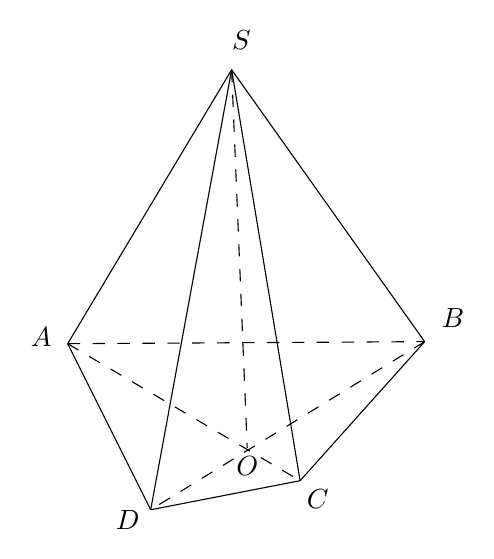
\begin{tikzpicture}[x=0.75pt,y=0.75pt,yscale=-1,xscale=1]
					\draw [color={rgb,255:red,0; green,0; blue,0},draw  opacity=1] [dash pattern={on 4.5pt off 4.5pt}] (152,176) -- (324,175);
					 \draw [color={rgb,255:red,0; green,0; blue,0},draw opacity=1] (152,176) -- (192,256);
					\draw [color={rgb,255:red,0; green,0; blue,0},draw opacity=1]  (324,175) -- (264,242);
					\draw [color={rgb,255:red,0; green,0; blue,0},draw  opacity=1] (192,256) -- (264,242);
					\draw [color={rgb,255:red,0; green,0;  blue,0},draw opacity=1] (231,44) -- (152,176);
					\draw [color={rgb,255:red,0; green,0; blue,0},draw opacity=1] (231,44) -- (192,256); 
					\draw  [color={rgb,255:red,0; green,0; blue,0},draw opacity=1] (231,44) -- (264,242);
					 \draw [color={rgb,255:red,0; green,0; blue,0},draw opacity=1] (231,44) -- (324,175);
					\draw [dash pattern={on 4.5pt off  4.5pt}] (152,176) -- (264,242);
					\draw [dash pattern={on 4.5pt off  4.5pt}] (324,175) -- (192,256);
					\draw [dash pattern={on 4.5pt off 4.5pt}]  (231,44) -- (238.51,226.23);
					\draw (230,24) node  [anchor=north west][inner sep=0.75pt] [align=left] {$S$};
					\draw (133,167) node  [anchor=north west][inner sep=0.75pt] [align=left] {$A$};
					\draw (331,158) node [anchor=north west][inner  sep=0.75pt] [align=left] {$B$};
					\draw (174,255) node [anchor=north  west][inner sep=0.75pt] [align=left] {$D$};
					\draw (266,245)  node [anchor=north west][inner sep=0.75pt] [align=left] {$C$};
					\draw (232,229) node [anchor=north  west][inner sep=0.75pt] [align=left] {$O$};
				\end{tikzpicture}
		\end{center}
	 }
\end{ex}

% nguồn: Ok_TraLoiNgan_Lop11_Lan1
\begin{ex}%[1H4V2-3]%[ma:4f0b24d8]
	Cho hình chóp $S.ABCD$ có đáy $ ABCD $ là hình thoi tâm $ I $. Gọi $ M $ là trung điểm của $ CD $. Trên cạnh $ SM $ lấy điểm $ N $ sao cho $ SN=\dfrac{1}{3}SM $. Giao tuyến của  hai mặt phẳng $ (NAD) $ và $ (NBC) $ cắt $ SI $ tại $ P $. Tính $ \dfrac{SP}{PI} \cdot \dfrac{SN}{NM} $.
	 \shortans{0,25}
	\loigiai{ 
	\immini{Ta  có $\heva{
		&AD\parallel BC\\ &(NAD)\cap (NBC)=NP.}$\\ 
		 Suy ra $NP\parallel AD$.\\
		 Mặt khác $ IM\parallel AD $. Do đó, $ IM\parallel NP $.\\
		Suy ra, $  \dfrac{SP}{SI}=\dfrac{SN}{SM}=\dfrac{1}{3} $.\\
		 Vậy $ \dfrac{SP}{PI}\cdot\dfrac{SN}{NM}=\dfrac{1}{2}\cdot\dfrac{1}{2}=\dfrac{1}{4}=0{,}25$.
		}{ 
		\begin{tikzpicture}[scale=0.6,line join = round,line cap = round,font=\footnotesize]
				\tikzset{label  style/.style={font=\footnotesize}}
				\coordinate[label  = right:$C$] (C) at (7,0);
				 \coordinate[label = left:$A$] (A) at (3,3);
				\coordinate[label = left:$B$] (B) at  (0,0);
				 \coordinate[label = right:$D$] (D) at ($(A)+(C)-(B)$);
				\coordinate  (H) at ($(A)!0.3!(C)$);
				\coordinate[label =  above:$S$] (S) at ($(H)+(0,6)$);
				\coordinate[label = left:$I$] (I) at  ($(C)!0.5!(A)$);
				\coordinate[label = right:$M$]  (M) at ($(C)!0.5!(D)$);
				 \coordinate[label = right:$N$] (N) at ($(S)!0.33!(M)$);
				\coordinate[label =  left:$P$] (P) at ($(S)!0.33!(I)$);
				\draw  (S)--(D)--(C)--(B)--cycle (S)--(C)
					 (S)--(M);
				\draw[dashed]  (A)--(S)
					 (A)--(D)
					 (A)--(B)
					 (I)--(S)
					(N)--(P) 
					(M)--(I); 
				\foreach \diem in {B,C,A,D,S,M,N,P,I}\fill  (\diem) circle (1pt);
			\end{tikzpicture}
		} 
	 }
\end{ex}

% nguồn: Ok_TraLoiNgan_Lop11_Lan1
\begin{ex}%[1H4V2-3]%[ma:d9d17be8]
	Cho hình chóp $S.ABCD$, trong đó $ABCD$ là một hình thang với đáy $AB$ và $CD$. Gọi $I$ và $J$ lần lượt là trung điểm của $AD$ và $BC$, $G$ là trọng  tâm của tam giác $SAB$. Giao tuyến $d$ của hai mặt phẳng $(SAB)$ và $(GIJ)$. Biết $d$ cắt $SA$ tại $M$ và cắt $SB$ tại $N$. Tứ giác $MNJI$ là hình bình hành thì $AB=kCD$. Khi đó giá trị của $k$ bằng bao nhiêu?
	\shortans{3} 
	 \loigiai{
		\begin{center}
			\begin{tikzpicture}[line join=round,line cap=round,>=stealth,scale=0.65,font=\footnotesize]
					\foreach \x/\y/\n in {0/0/A,2/-2/D,6/0/B}  \coordinate (\n) at (\x,\y);
					\coordinate (C) at ($(D)+(0:3)$); 
					\coordinate (S) at  ($(A)+(2.5,4)$);
					 \coordinate (I) at ($(A)!1/2!(D)$);
					\coordinate (J)  at ($(B)!1/2!(C)$);
					 \coordinate (K) at ($(B)!1/2!(A)$);
					\coordinate  (G) at ($(S)!2/3!(K)$);
					\coordinate (M) at  ($(S)!2/3!(A)$);
					 \coordinate (N) at ($(S)!2/3!(B)$);
					 \draw (S)--(A)--(D)--(C)--(B)--(S)--(C)
						(S)--(D) 
						 (M)--(I)
						(N)--(J); 
					\draw[dashed]  (A)--(B)
						(G)--(I)--(J)--(G) 
						(M)--(N); 
					 \foreach \t/\g in {A/150,D/-150,C/-30,B/30,S/90,M/160,N/60,G/50,I/-120,J/-30}{
						\draw[fill=black] (\t)  circle (1pt) node[shift={(\g:7pt)}]{$ \t $};
					 }
				\end{tikzpicture}
		\end{center}
		\begin{itemize}
			\item Tìm giao tuyến $d$ của  $(SAB)$ và $(GIJ)$:\\
			 Dễ thấy $G \in(SAB) \cap(GIJ) \Rightarrow G \in d$ với $d=(SAB) \cap(GIJ)$.\\
			$IJ$  là đường trung bình của hình thang $ABCD$ nên $IJ \parallel AB$.\\
			Ta có $\heva{&d=(SAB) \cap(GIJ) \\& AB \parallel  IJ \\ &AB \subset(SAB), IJ \subset(GIJ)} \Rightarrow d \parallel AB \parallel IJ$.\\
			Vậy giao tuyến  $d$ của hai mặt phẳng $(SAB)$ và $(GIJ)$ là đường thẳng $d$ qua $G$ và song song với đường thẳng $AB$.
			\item Tìm điều kiện  của $AB$ và $CD$ để $MNJI$ là hình bình hành:\\
			Gọi $E$ là trung điểm  $AB$.\\
			Ta có 
			$MN \parallel IJ$; $MNJI$ là hình bình hành khi và chỉ khi $MN=IJ$.\quad  (1)\\
			Vì $MG \parallel AE \Rightarrow \dfrac{SM}{SA}=\dfrac{SG}{SE}=\dfrac{2}{3}$ ($G$ là trọng tâm của tam giác  $SAB$).\\
			Vì $MN \parallel AB  \Rightarrow \dfrac{MN}{AB}=\dfrac{SM}{SA}=\dfrac{2}{3} \Rightarrow MN=\dfrac{2}{3} AB$.\quad (2)\\
			Vì  $IJ$ là đường trung bình của hình thang $ABCD$ nên $IJ=\dfrac{AB+CD}{2}$.\quad (3)\\
			Từ  (1), (2), (3), ta có
			 $\dfrac{2}{3} AB=\dfrac{A B+C D}{2} \Leftrightarrow 4AB=3AB+3CD \Leftrightarrow AB=3CD$.
		\end{itemize}
		Vậy với hình chóp ban đầu có $AB=3CD$ thì  $MNJI$ là hình bình hành. Suy ra $k=3$.
	 }
\end{ex}

% nguồn: Ok_TraLoiNgan_Lop11_Lan1
\begin{ex}%[1H4V2-3]%[ma:7e9bc768]
	Cho tứ diện $ ABCD$ và $ M$ là một điểm bên trong $\triangle ABC,N$ là điểm bên trong của $\triangle ACD$. Gọi $ E=AM\cap BC$; $ F=AN\cap CD$ và $ G=DN\cap  AC$.\\
	a) đường thẳng $a$ là giao tuyến của $ (AMN)$ và $ (BCD)$\\ 
	 b) đường thẳng $b$ là giao tuyến của $ (DMN)$ và $ (ABC)$.\\
	nếu $a$ và $b$ đồng phẳng thì chọn $0$, trùng nhau chọn $1$, chéo nhau chọn $2$, không nằm ở trường hợp nào của các lựa chọn trước  thì chọn $3$.
	 \shortans{2}
	\loigiai{ 
		a)  Tìm giao tuyến của $ (AMN)$ và $ (BCD)$ :\\
		Trong mặt phẳng $ (ABC)$, gọi $  E=AM\cap BC$;\\
		Trong mặt phẳng $ (ACD)$, gọi $  F=AN\cap CD$.\\
		Ta có  $\heva{
		{E\in AM,AM\subset (AMN)}\\ 
		{E\in BC,BC\in  (BCD)}
		}$\\ 
		$\Rightarrow E\in  (AMN)\cap (BCD).\quad(1)$\\
		 Tương tư$\heva{
		{F\in AN,AN\subset (AMN)}\\ 
		 {F\in CD,CD\in (BCD).}
		}$\\ 
		$\Rightarrow F\in (AMN)\cap  (BCD).\quad (2)$\\
		Từ $(1)$  và $(2)$ suy ra $ EF=(AMN)\cap (BCD)$.
		\begin{center}
			 \tikzset{every picture/.style={line width=0.75pt}}
			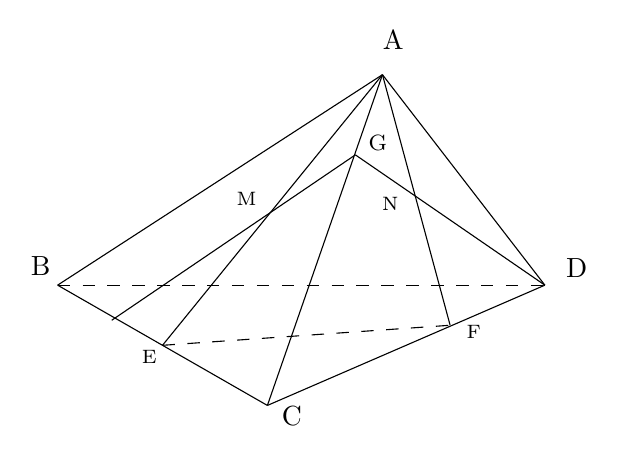
\begin{tikzpicture}[x=0.75pt,y=0.75pt,yscale=-1,xscale=1]
					\draw [dash pattern={on 4.5pt off 4.5pt}] (108.04,150.99) -- (342.81,150.99); 
					\draw (108.04,150.99)  -- (209.12,208.94);
					\draw (342.81,150.99)  -- (209.12,208.94);
					\draw  (108.04,150.99) -- (264.55,49.58);
					\draw  (209.12,208.94) -- (264.55,49.58);
					\draw (342.81,150.99) -- (264.55,49.58); 
					\draw (264.55,49.58)  -- (158.58,179.97);
					\draw (264.55,49.58) --  (297.16,170.31);
					\draw [dash pattern={on  4.5pt off 4.5pt}] (158.58,179.97) -- (297.16,170.31);
					 \draw (342.81,150.99) -- (251.51,88.21);
					 \draw (251.51,88.21) -- (134.13,167.9);
					\draw (263.45,27.2) node [anchor=north west][inner sep=0.75pt]  [align=left] {A};
					\draw (256.61,77.49) node [anchor=north west][inner sep=0.75pt] [font=\footnotesize] [align=left] {G}; 
					\draw (214.85,208.29) node  [anchor=north west][inner sep=0.75pt] [align=left] {C};
					\draw (93.89,135.85) node  [anchor=north west][inner sep=0.75pt] [align=left] {B};
					 \draw (351.8,137.06) node [anchor=north west][inner sep=0.75pt] [align=left] {D};
					\draw  (147.38,181.11) node [anchor=north west][inner sep=0.75pt] [font=\scriptsize] [align=left] {E};
					\draw (303.89,169.04)  node [anchor=north west][inner sep=0.75pt] [font=\scriptsize] [align=left] {F};
					\draw (263.13,107.46)  node [anchor=north west][inner sep=0.75pt] [font=\scriptsize] [align=left] {N};
					\draw (193.03,105.05) node [anchor=north west][inner sep=0.75pt] [font=\scriptsize] [align=left]  {M};
				\end{tikzpicture}
		\end{center}
		 b) Tìm giao tuyến của $ (DMN)$ và $ (ABC)$ :\\
		Ta có  $ M\in AE,AE\subset (ABC)\Rightarrow M\in (ABC)\Rightarrow M\in (ABC)\cap (DMN)$.(3)\\
		 Trong mặt phẳng $ (ACD)$, gọi $ G=DN\cap AC$.\\
		Ta  có $\heva{
		{G\in AC,AC\subset (ABC)}\\ 
		{G\in DN,DN\subset  (DMN).}
		}\Rightarrow G\in (ABC)\cap (DMN).\,(4)$\\ 
		Từ $(3)$ và $(4)$ suy  ra $ MG=(DMN)\cap (ABC)$.
	} 
\end{ex}

% nguồn: Ok_TraLoiNgan_Lop11_Lan1
\begin{ex}%[1H4V2-3]%[ma:37e24363]
	Cho hai hình bình hành $ABCD$ và $ABEF$ không cùng nằm trong một mặt phẳng. Trên cạnh $AC$ lấy điểm $M$ và trên cạnh $BF$ lấy điểm $N$ sao cho 
	 $\dfrac{AM}{AC} = \dfrac{BN}{BF} = k$ Tìm $k$ để $MN \parallel DE$.
	 (Làm tròn kết quả đến hàng phần trăm).
	 \shortans{0,33}
	\loigiai{\begin{center}
		\begin{tikzpicture}[scale=0.8,font=\footnotesize,line join=round,line cap=round,>=stealth]
				 \path
					(0,0)  coordinate (A)
					 ++(-45:3) coordinate (F)
					++(0:6) coordinate (E) 
					($(A)+(E)-(F)$) coordinate  (B)
					++(+75:3) coordinate (C) 
					($(A)+(C)-(B)$) coordinate (D) 
					($(A)!1/3!(B)$)  coordinate (I);
				\path[name path =  di] (D)--(I);
				\path[name path = ac]  (A)--(C);
				\path[name intersections =  {of = ac and di}] (intersection-1) coordinate (M);
				\path[name path  = ei] (E)--(I);
				\path[name  path = bf] (B)--(F);
				\path[name intersections = {of =  bf and ei}] (intersection-1) coordinate (N);
				\draw  (A)--(B)--(C)--(D)--cycle;
				\draw 
					(A)--(F)--(E)--(B) 
					 (D)--(E)--(I)--(D)
					(A)--(C) 
					 (B)--(F)
					(M)--(N); 
				 \foreach \i/\g in {A/180,B/0,C/90,D/90,F/-90,E/-90,I/-90,M/150,N/-90}
				\fill[black] (\i) circle (1pt)+(\g:5mm) node[scale=1]{$\i$}; 
			\end{tikzpicture}
	\end{center}
	 \noindent
	Ta có: $MN \parallel DE$ nên bốn điểm $M, N, D, E$ đồng  phẳng.\\
	Trong mặt phẳng $(MNED)$, gọi $I = DM \cap NE \Rightarrow I \in AB$  (3 giao tuyến đồng quy).\\
	Hơn  nữa, $MN \parallel NE$, nên $\dfrac{IM}{DM} = \dfrac{IN}{NE}$.\\
	Theo giả  thiết, ta có:
	$\dfrac{AM}{AC} = k  \quad (1)$.\\
	$\Rightarrow \dfrac{AC-MC}{AC} = k \Rightarrow 1-\dfrac{MC}{AC} =  k \Rightarrow \dfrac{MC}{AC} = 1 - k \quad (2)$.\\
	Từ (1) và (2) suy ra $\dfrac{AM}{MC} = \dfrac{k}{1-k}$; tương tự ta chứng minh được  $\dfrac{BN}{FN} = \dfrac{k}{1-k}$.\\
	Vì $AB \parallel CD$ nên  $\dfrac{IM}{DM}=\dfrac{IA}{DC} = \dfrac{AM}{MC} = \dfrac{k}{1-k}$.\\
	Vì $AB \parallel EF$  nên $\dfrac{IN}{NE} = \dfrac{BI}{EF} = \dfrac{BN}{NF} = \dfrac{k}{1-k}$.\\
	Mặt khác $\dfrac{AI}{DC} + \dfrac{BI}{EF} = \dfrac{AI}{FE} + \dfrac{BI}{EF} = 1 \Rightarrow  2 \cdot \dfrac{k}{1-k} = 1$.\\
	$\Rightarrow 2 k = 1-k \Rightarrow k=\dfrac{1}{3}$.\\ 
	Vậy với $k = \dfrac{1}{3}$ thì $MN  \parallel DE$.
 }
\end{ex}

% nguồn: Ok_TraLoiNgan_Lop11_Lan1
\begin{ex}%[1H4C2-3]%[ma:ed4124b7]
	Cho hình chóp $S.ABCD$ có đáy $ABCD$ là hình bình hành. Gọi $d$ là giao tuyến  của hai mặt phẳng $(SAD)$ và $(SBC)$. Gọi $M$ là trung điểm của $BC$, $N$ là điểm thuộc cạnh $SC$ sao cho $\dfrac{SN}{SC}=\dfrac{1}{4}$. Gọi $E$ là giao điểm của $MN$ và $d$, $F$ là giao điểm của $AE$ và $SD$. Tính tỉ số $t=\dfrac{S_{FDA}}{S_{FSE}}$?
	 \shortans{36}
	 \loigiai{
	\immini{Ta có $\heva{& AD\subset (SAD) \\& BC\subset  (SBC) \\& AD\parallel BC}$\\
		$\Rightarrow (SAD)\cap (SBC)=d\parallel AD$.\\ 
		Dễ thấy  $\triangle CMN\sim \triangle SEN$, ta có $$\dfrac{SE}{CM}=\dfrac{SN}{CN}=\dfrac{1}{3}.$$
		 Suy ra $SE=\dfrac{1}{3}CM=\dfrac{1}{6}BC=\dfrac{1}{6}AD$.\\
		Trong $(SAD)$ có $\triangle SEF\sim \triangle DAF$.  Khi đó $$\dfrac{FS}{FD}=\dfrac{FE}{FA}=\dfrac{SE}{AD}=\dfrac{1}{6}.$$
		}{\begin{tikzpicture}[scale=1,font=\footnotesize,line join=round,line cap=round,>=stealth]
		 \def\bc{5}
		 \def\ba{2}
		 \def\h{4}
		 \def\gocB{40}
		 \path
			 (0,0) coordinate (B)
			 (\gocB:\ba) coordinate (A)
			 (\bc,0) coordinate (C)
			 ($(C)-(B)+(A)$) coordinate (D)
			 ($(A)+(80:\h)$) coordinate (S)
			 ($(B)!1/2!(C)$) coordinate (M)
			($(S)!1/4!(C)$) coordinate (N); 
		\draw ($(S)+(0:\bc)$) coordinate (S1) node[below left]{$d$}--($(S)+(180:\bc/3)$) coordinate  (S2);
		\path (intersection of M--N and S1--S2)  coordinate (E);
		\path (intersection of A--E  and S--D) coordinate (F);
		\path (intersection of M--N and S--D) coordinate (J); 
		\draw (B)--(C)--(S)--cycle  (J)--(D)--(C)
			(M)--(E); 
		\draw[dashed]  (E)--(A)--(D)
			(S)--(A)--(B) 
			(J)--(S); 
		\foreach \x/\g in {A/160,B/-145,C/-45,D/0,S/90,M/-90,N/0,E/90,F/90}\fill  (\x) circle (1pt)+(\g:3mm) node[black]{$ \x $};
	\end{tikzpicture}
		} 
		\noindent Do đó $t=\dfrac{S_{FDA}}{S_{FSE}}=\dfrac{\dfrac{1}{2}FD\cdot FA\cdot\sin {AFD}}{\dfrac{1}{2}FS\cdot FE\cdot \sin {SFE}} = \dfrac{FD \cdot FA}{FS \cdot FE}=\dfrac{FD}{FS}\cdot\dfrac{FA}{FE}=36$. 
	 }
\end{ex}


%%%%%%%%%%%%%%%% TỰ LUẬN %%%%%%%%%%%%%%%%

% nguồn: Ok_TuanLuan_Toan11_Lan2
\begin{ex}%[1H4N2-3]%[ma:75365d0f]
	Cho hình hộp $ABCD.A'B'C'D'$ (hình vẽ bên). Chứng minh rằng các đường chéo $AC'$, $BD'$, $CA'$ và $DB'$ của hình hộp cùng đi  qua trung điểm của mỗi đường.
	\begin{center}
		\begin{tikzpicture}[scale=0.8,font=\footnotesize,line join=round,line cap=round,>=stealth]
				\coordinate  (A) at (0,0);
				\coordinate (D) at  (-2,-2);
				\coordinate (B)  at (6,0);
				 \coordinate (C) at ($(B)+(D)-(A)$);
				\foreach \i in {A,B,C,D}{\coordinate (\i') at  ($(\i)-(0,4)$);}
				\draw  (A)--(B)--(C)--(D)--cycle;
				 \draw (B)--(B')
					 (C)--(C')
					(D)--(D') 
					(B')--(C')--(D'); 
				 \draw[dashed](B')--(A')--(A)
					(A')--(D') 
					 (A)--(C')
					(D)--(B'); 
				\foreach \i/\g in {A'/170,B'/20,C'/-90,D'/-90,A/90,B/90,C/-20,D/180}{\draw[fill=blue](\i) circle (1pt) 
					 ($(\i)+(\g:5mm)$) node[scale=1]{$\i$};}
			\end{tikzpicture}
	\end{center}
	 \loigiai{
		Đáy $ABCD$ của hình hộp là  hình bình hành nên $AD \parallel BC$ và $AD=BC$.\\
		Mặt bên $BCC'B'$ của hình hộp là  hình bình hành nên $BC \parallel B'C'$ và $BC=B'C'$.\\
		Vậy $AD \parallel B'C'$ và $AD=B'C'$  suy ra $ADC'B'$ là hình bình hành.\\
		 Từ đó $AC'$ và $DB'$ cắt nhau tại trung điểm của mỗi đường.\\
		Tương tự  $AC'$ và $BD'$, $AC'$ và $CA'$ cũng cắt nhau tại trung điểm của mỗi đường.\\
		Vậy bốn  đường chéo của hình hộp cùng đi qua trung điểm của mỗi đường.
	 }
\end{ex}

% nguồn: Ok_TuanLuan_Toan11_Lan2
\begin{ex}%[1H4N2-3]%[ma:21d49049]
	Cho hình chóp $S.ABCD$ có đáy $ABCD$ là hình thang với $AB \parallel CD$. Xác định giao tuyến của hai mặt phẳng  $(SAB)$ và $(SCD)$.
	\begin{center}
		\begin{tikzpicture}[scale=0.8,font=\footnotesize,line join=round,line cap=round,>=stealth]
				\coordinate  (A) at (0,0);
				\coordinate (B) at  (5,0);
				\coordinate (C)  at (3,-2);
				 \coordinate (D) at (1,-2);
				\coordinate (S)  at ($(A)+(1,5)$);
				\coordinate (x) at ($(S)+(-1,0)$);  \coordinate (y) at ($(S)+(3,0)$);
				\draw (D)--(A)--(S)--(B) 
					 (S)--(C)--(D)--(S)
					(B)--(C); 
				\draw  (x)--(y) node[above]{$d$};
				\draw[dashed](A)--(B); 
				\foreach \i/\g in {S/90,A/180,B/00,C/-90,D/-90}{\draw[fill](\i) circle  (1pt)
					($(\i)+(\g:3mm)$)  node[scale=1]{$\i$};}
			\end{tikzpicture}
	\end{center}
	\loigiai{ 
	Hai mặt phẳng $(SAB)$ và $(SCD)$ có điểm chung là $S$ và lần lượt chứa hai đường thẳng $AB$ và $CD$ song song với  nhau nên giao tuyến của hai mặt phẳng đó là đường thẳng $d$ đi qua $S$ và song song với $AB$ và $CD$.
	} 
\end{ex}

% nguồn: Ok_TuanLuan_Toan11_Lan2
\begin{ex}%[1H4N2-3]%[ma:f9ad1c6a]
	Cho hình chóp $S.ABCD$ có đáy  $ABCD$ là hình bình hành. Xác định giao tuyến của hai mặt phẳng $(SAB)$ và $(SCD)$.
	\begin{center}
		\begin{tikzpicture}[scale=0.8,font=\footnotesize,line join=round,line cap=round,>=stealth]
				\coordinate (D)  at (0,0);
				\coordinate (C) at  (5,0);
				 \coordinate (A) at (1,-2);
				\coordinate (B) at  ($(A)+(C)-(D)$);
				\coordinate  (S) at ($(A)+(1,5)$);
				\coordinate (x) at  ($(S)+(-1,0)$); \coordinate (y) at ($(S)+(3,0)$);
				\draw  (A)--(D)--(A)--(B)--(S)--(C)--(B)
					 (A)--(S)--(D);
				\draw (x)--(y) node[above]{$m$}; 
				 \draw[dashed](C)--(D);
				\foreach \i/\g in {S/90,A/-90,B/-90,C/0,D/180}{\draw[fill](\i)  circle (1pt)
					 ($(\i)+(\g:3mm)$) node[scale=1]{$\i$};}
			\end{tikzpicture}
	\end{center}
	 \loigiai{
	Mặt phẳng $(SAB)$ và $(SCD)$ có điểm chung $S$ và chứa  hai đường thẳng song song là $AB$ và $CD$.\\
	Do đó, giao tuyến của hai mặt phẳng $(SAB)$ và $(SCD)$ là  đường thẳng $m$ đi qua $S$ và song song với $AB$, $CD$.
	 }
\end{ex}

% nguồn: Ok_TuanLuan_Toan11_Lan2
\begin{ex}%[1H4N2-3]%[ma:8bc90882]
	Cho hình chóp  $S.ABCD$ có đáy là hình bình hành. Xác định giao tuyến của hai mặt phẳng $(SBC)$ và $(SAD)$.
	\begin{center}
		\begin{tikzpicture}[scale=0.8,font=\footnotesize,line join=round,line cap=round,>=stealth]
				\coordinate (A)  at (0,0);
				 \coordinate (D) at (5,0);
				 \coordinate (B) at (-2,-2);
				\coordinate (C) at ($(B)+(D)-(A)$); 
				\coordinate (S) at ($(A)+(1,4)$); 
				\coordinate (x) at ($(S)+(-1,0)$);  \coordinate (y) at ($(S)+(3,0)$);
				\draw  (B)--(S)--(C)--(D)--(S)
					 (B)--(C);
				 \draw (x)--(y) node[above]{$d$};
				\draw[dashed](B)--(A)--(S) 
					 (D)--(A);
				 \foreach \i/\g in {S/90,A/-90,B/-90,C/-90,D/0}{\draw[fill](\i) circle (1pt)
					 ($(\i)+(\g:3mm)$) node[scale=1]{$\i$};}
			\end{tikzpicture}
	\end{center}
	\loigiai{ 
		Mặt phẳng $(SBC)$ và $(SAD)$  có điểm chung $S$, chứa hai đường thẳng song song $BC$ và $AD$.\\
		Suy ra hệ quả của định lí 2, giao tuyến của $(SBC)$  và $(SAD)$ là đường thẳng $d$ đi qua $S$ và song song với $BC$ và $AD$.
	} 
\end{ex}

% nguồn: Ok_TuanLuan_Toan11_Lan2
\begin{ex}%[1H4H2-3]%[ma:49b356e2]
	Cho tứ diện $ABCD$. Gọi $M$, $N$ lần lượt là trung điểm của các cạnh $BC$, $CD$ và $P$ là một điểm thuộc cạnh $AC$. Xác định giao tuyến của hai mặt phẳng $(AMN)$ và $(BPD)$ và chứng minh giao  tuyến đó song song với $BD$.
	\loigiai{ 
		\begin{center}
			\begin{tikzpicture}[scale=1,font=\footnotesize,line join=round,line cap=round,>=stealth]
					\coordinate (B) at (0,0);  \coordinate (C) at (1.5,-2); \coordinate (D) at (6,0); \coordinate (A) at ($(B)+(2,4)$);
					\coordinate  (M) at ($(C)!1/2!(B)$); \coordinate (N) at ($(C)!1/2!(D)$); \coordinate (P) at ($(A)!1/3!(C)$);
					\coordinate (E) at (intersection of B--P and A--M); 
					\coordinate (F) at (intersection  of D--P and A--N);
					 \draw (A)--(B)--(C)--(A)--(D)--(C)
						(N)--(A)--(M) 
						 (B)--(P)--(D);
					 \draw[dashed] (B)--(D)
						 (E)--(F)
						(M)--(N); 
					\foreach \x/\g in {A/90,B/180,C/-90,D/0,E/120,F/50,M/-120,N/-60,P/50} \fill (\x) circle  (1pt)
						($(\x)+(\g:3mm)$)  node{$\x$};
				\end{tikzpicture}
		\end{center}
		Trong  mặt phẳng $(AMN)$ gọi $E=AM\cap BP$.\\
		Khi đó $\heva{&E\in BP\subset (BPD)\\& E\in AM\subset (AMN)} \Rightarrow E\in (AMN) \cap (BPD)$  (1).\\
		Trong mặt phẳng $(ACD)$ gọi $F=AN\cap PD$.\\ 
		Khi đó $\heva{&F\in AN\subset (AMN) \\& F\in PD\subset (BPD)} \Rightarrow F\in (AMN)  \cap (BPD)$ (2).\\
		Từ (1) và (2) suy ra $(AMN) \cap  (BPD)=EF$.\\
		Xét  tam giác $BCD$ có $M$, $N$ lần lượt là trung điểm của $BC$ và $CD\Rightarrow MN\parallel BD$.\\
		Mặt khác $BD\subset (BPD)$; $MN\subset (AMN)$  và $(BPD) \cap (AMN)=EF$.\\
		Vậy  $MN\parallel EF\parallel BD$.
	} 
\end{ex}

% nguồn: Ok_TuanLuan_Toan11_Lan2
\begin{ex}%[1H4H2-3]%[ma:54a6f83b]
	Cho hình chóp $S.ABCD$ có đáy $ABCD$ là  hình thang ($AB\parallel CD$). Gọi $M$ là trung điểm của đoạn thẳng $SD$.
	\begin{enumEX}{1}
		\item  Xác định giao tuyến của mặt phẳng $(MAB)$ và $(SCD)$.
		\item Gọi $N$ là giao điểm  của đường thẳng $SC$ và mặt phẳng $(MAB)$. Chứng minh rằng $MN$ là đường trung bình của tam giác $SCD$.
	\end{enumEX}
	 \loigiai{
		\begin{center}
			\begin{tikzpicture}[scale=1,font=\footnotesize,line join=round,line cap=round,>=stealth]
					\coordinate (D)  at (0,0);
					\coordinate (C) at  (5,0);
					\coordinate (A) at (1,-2); 
					\coordinate (B)  at (3,-2);
					\coordinate  (S) at ($(A)+(1,5)$);
					\coordinate  (M) at ($(S)!0.5!(D)$); \coordinate (N) at ($(S)!0.5!(C)$);
					\coordinate (y)  at ($(N)+(2,0)$);
					 \draw (A)--(B)--(C)--(S)--(D)--(A)--(S)--(B)--(N)
						 (A)--(M);
					\draw (N)--(y) node[above]{$x$}; 
					 \draw[dashed](C)--(D)
						 (B)--(M)--(N);
					\foreach \i/\g  in {S/90,A/-90,B/-90,C/0,D/180,M/150,N/70}{\draw[fill](\i) circle (1pt)
						($(\i)+(\g:3mm)$)  node[scale=1]{$\i$};}
				\end{tikzpicture}
		\end{center}
		\begin{enumEX}{1}
			\item Ta có $M\in SD\subset (SCD)$ và $M\in (MAB) \Rightarrow M\in  (SCD) \cap (MAB)$.\\
			Ta có $\heva{&CD\subset (SCD)\\& AB\subset  (MAB) \parallel CD\parallel AB}$\\
			 Vậy $(MAB) \cap (SCD)=Mx \parallel AB\parallel CD$.
			\item Theo đề bài, ta có $N$ là giao điểm của đường thẳng $SC$ và  mặt phẳng $(MAB)$.\\
			Suy ra $N\in (MAB)$ và $N\in  SC\subset (SCD)$.\\
			Mà  $(MAB) \cap (SCD)=Mx \parallel AB\parallel CD$.\\
			Suy ra $N\in Mx$ hay $MN\parallel  AB\parallel CD$.\\
			Xét tam giác $(SDC)$ ta có $\heva{&MS=MD\\& MN\parallel CD}  \Rightarrow NS=NC$.\\
			Vậy $MN$ là đường trung bình của tam  giác $SCD$.
		\end{enumEX}
	} 
\end{ex}

% nguồn: Ok_TuanLuan_Toan11_Lan2
\begin{ex}%[1H4H2-3]%[ma:c96e51b2]
	Cho hình chóp $S. ABCD$ đáy $ABCD$ là hình bình hành  tâm $H$. Mặt phẳng $(P)$ đi qua $H$ và song song với $(SAB)$. Tìm giao tuyến của
	\begin{enumerate}
		\item Mặt  phẳng $(P)$ và mặt phẳng $(ABCD)$.
		\item Mặt phẳng $(P)$  và mặt phẳng $(SBC)$.
	\end{enumerate}
	 \loigiai{
		\begin{center}
			\begin{tikzpicture}[line join = round,line cap = round,>=stealth,font=\footnotesize,scale=1,declare function={ab=2.5; ad=4.5; gs=80; sa=3; gocA=-130;}]
					\path 
						(0,0) coordinate (A) 
						 (ad,0) coordinate (D)
						(gocA:ab) coordinate (B) 
						 ($(D)-(A)+(B)$) coordinate (C)
						(gs:sa) coordinate  (S)
						(intersection  of A--C and B--D) coordinate (H)
						 ($(B)!0.5!(C)$) coordinate (E)
						 ($(S)!0.5!(C)$) coordinate (K)
						 ($(A)!0.5!(D)$) coordinate (F);
					\draw (S)--(B)--(C)--(D)--(S)--(C) 
						 (K)--(E);
					 \draw[dashed] (S)--(A)--(D)
						 (B)--(A)
						 (A)--(C)
						 (B)--(D)
						(E)--(F); 
					\foreach  \x/\gm in {A/150,B/180,C/-20,D/0,S/90,K/70,E/-90,F/50,H/-90} \fill (\x) circle (1pt)
						($(\x)+(\gm:3.5mm)$) node{$\x$}; 
				\end{tikzpicture}
		\end{center}
		\begin{enumerate}
			\item Giao tuyến của mặt phẳng $(P)$ và mặt phẳng  $(ABCD)$.\\
			Ta có $\heva{& (P) \parallel(SAB) \\ & \left(ABCD\right)\cap\left(SAB\right)=AB \\ & (P)\cap (ABCD)=H}\Rightarrow (P)\cap(ABCD)=EF$ với $\heva{& EF  \text{ qua } H \\ & EF\parallel AB \\ & E\in BC, F\in AD.}$
			\item Giao  tuyến của mặt phẳng $(P)$ và mặt phẳng $(SBC)$.
		\end{enumerate}
		Ta có $\heva{& (P)\parallel(SAB) \\ & (SBC)\cap (SAB)=SB \\ & (P)\cap (SBC)=E}\Rightarrow  (P)\cap (ABCD)=EK$ với $\heva{& EK\cap SC=K \\ & EK\parallel SB.}$
	 }
\end{ex}
